\chapter{Módulo 2: Microcontrolador}

\section{Paso 1:}

Instalar cristal de 20Mhz. X1

\begin{figure}[h]
	\centering
	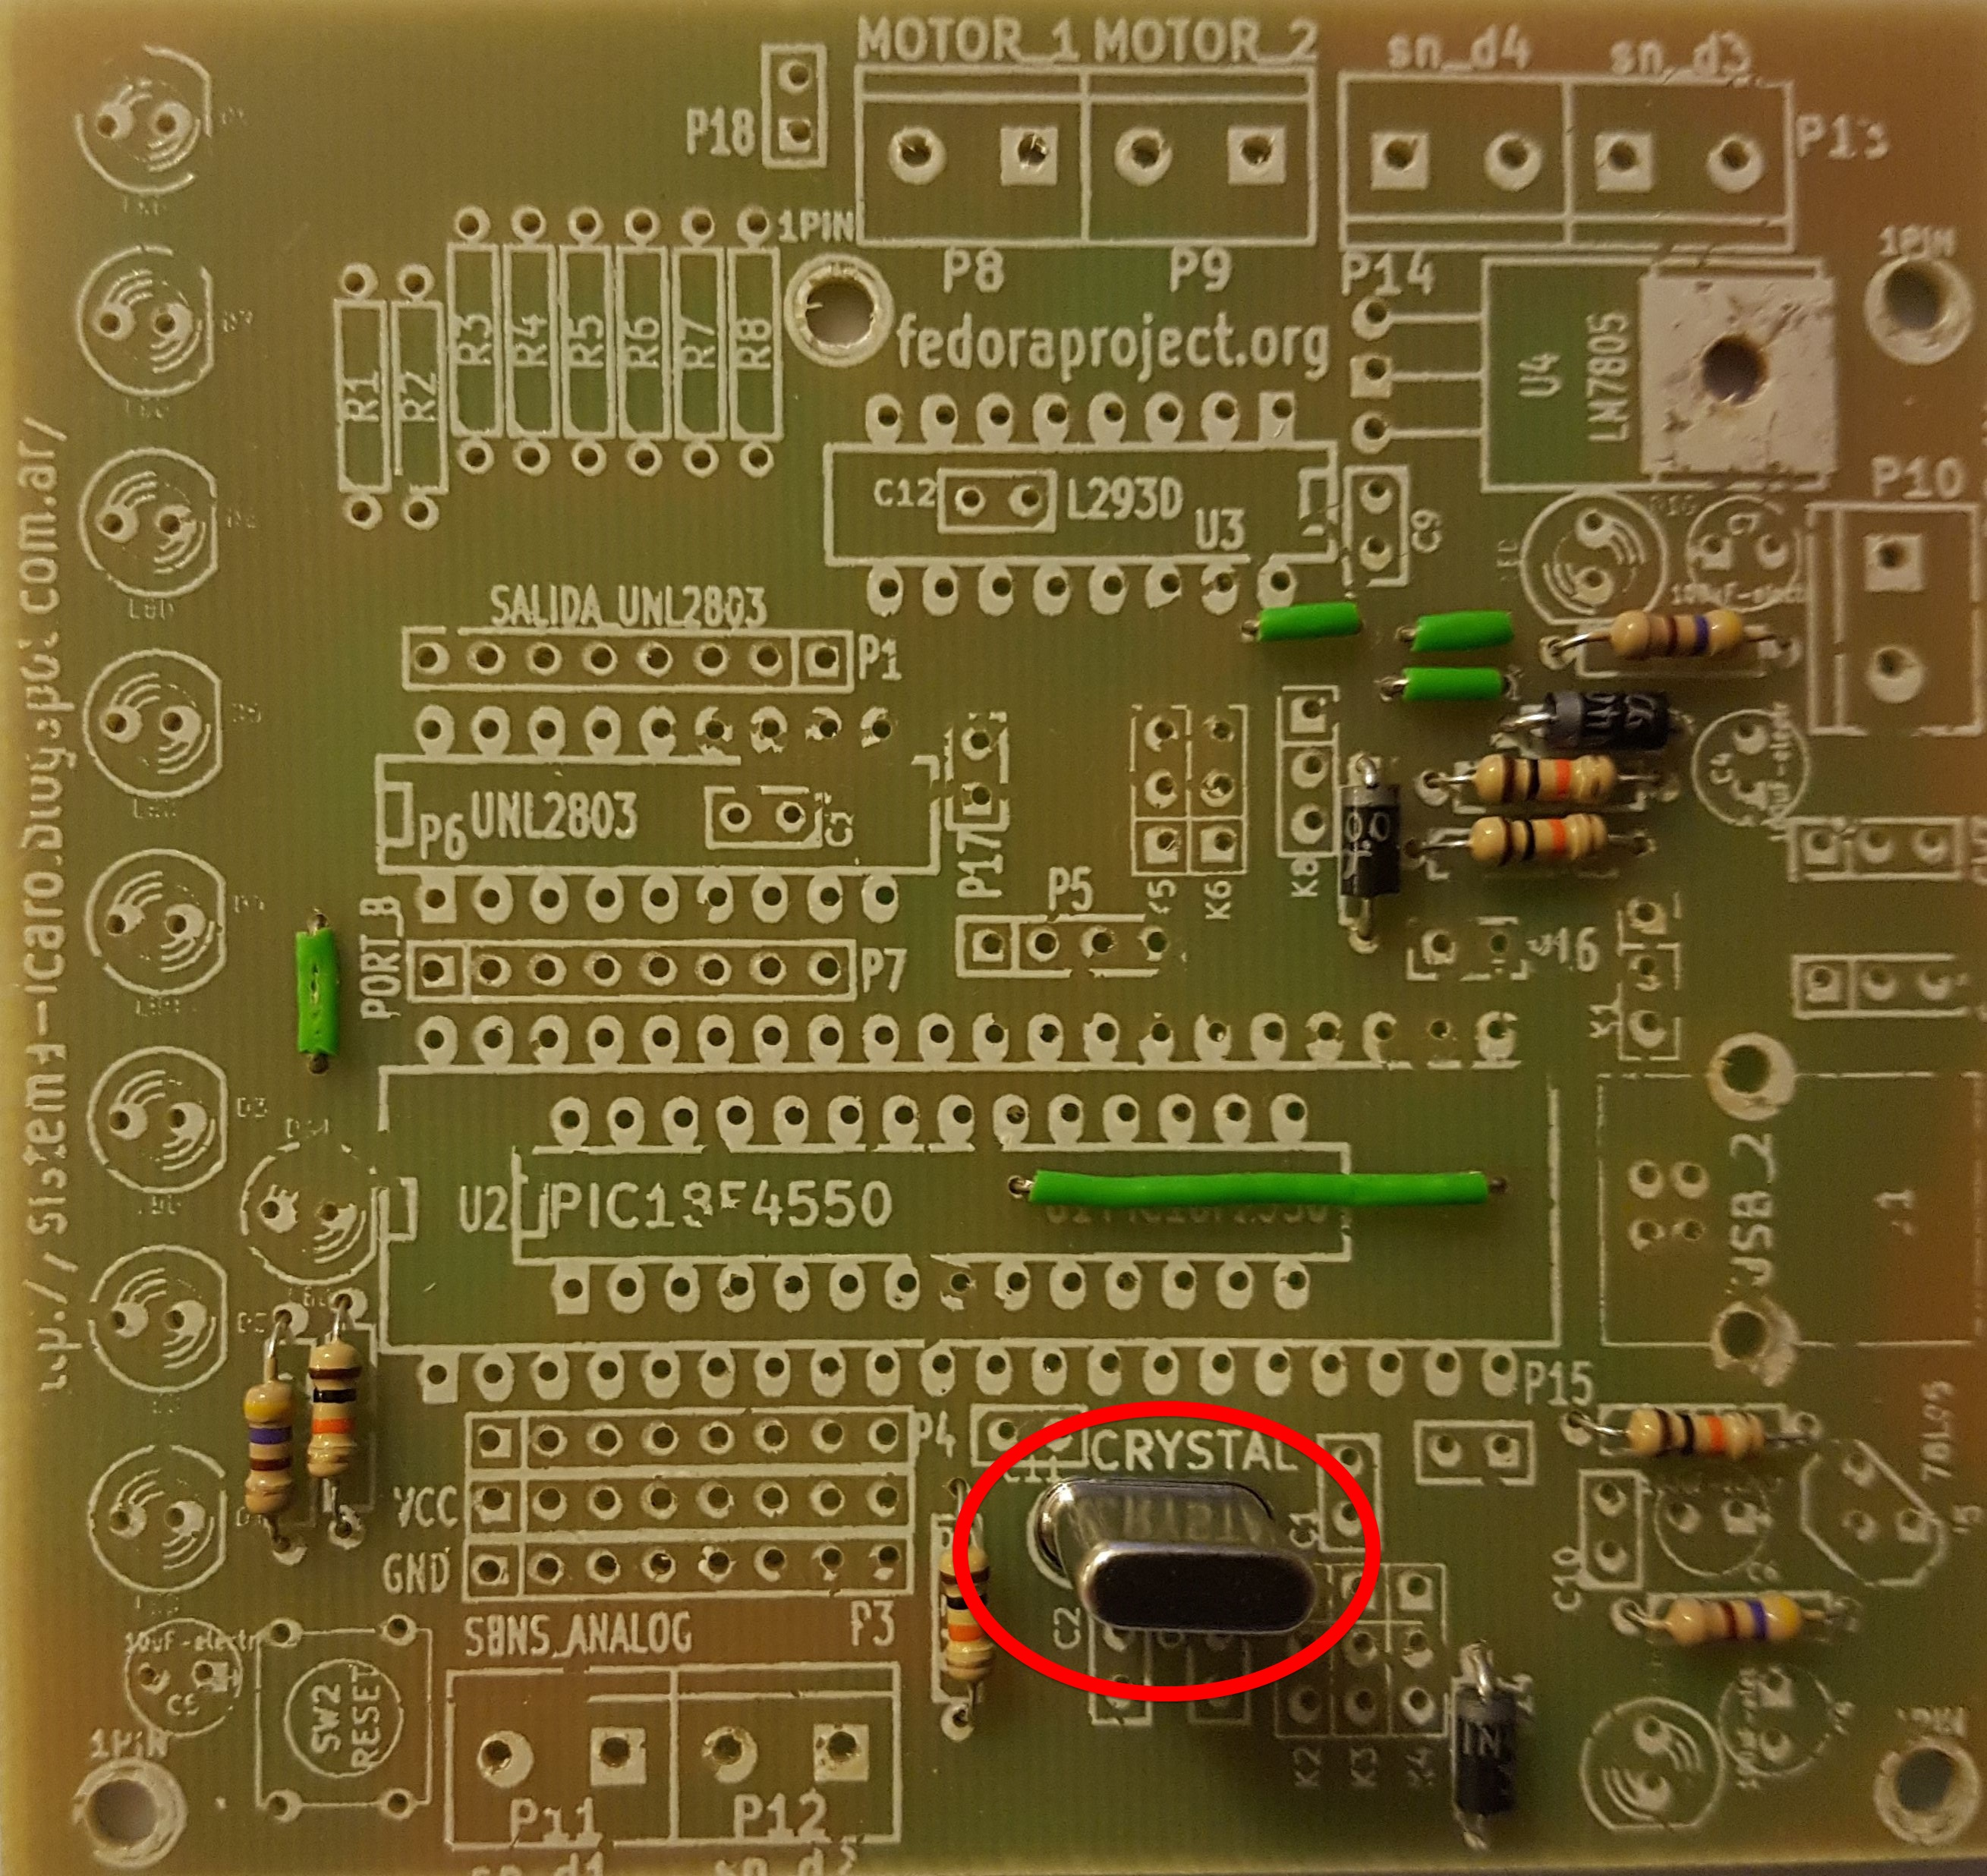
\includegraphics[width=0.8\linewidth]{Modulo_2/M2_1}
	\caption{Módulo 2 - Paso 1}
	\label{fig:M2_1}
\end{figure}

\newpage

\section{Paso 2:}

Push Botón (Reset). SW2

\begin{figure}[h]
	\centering
	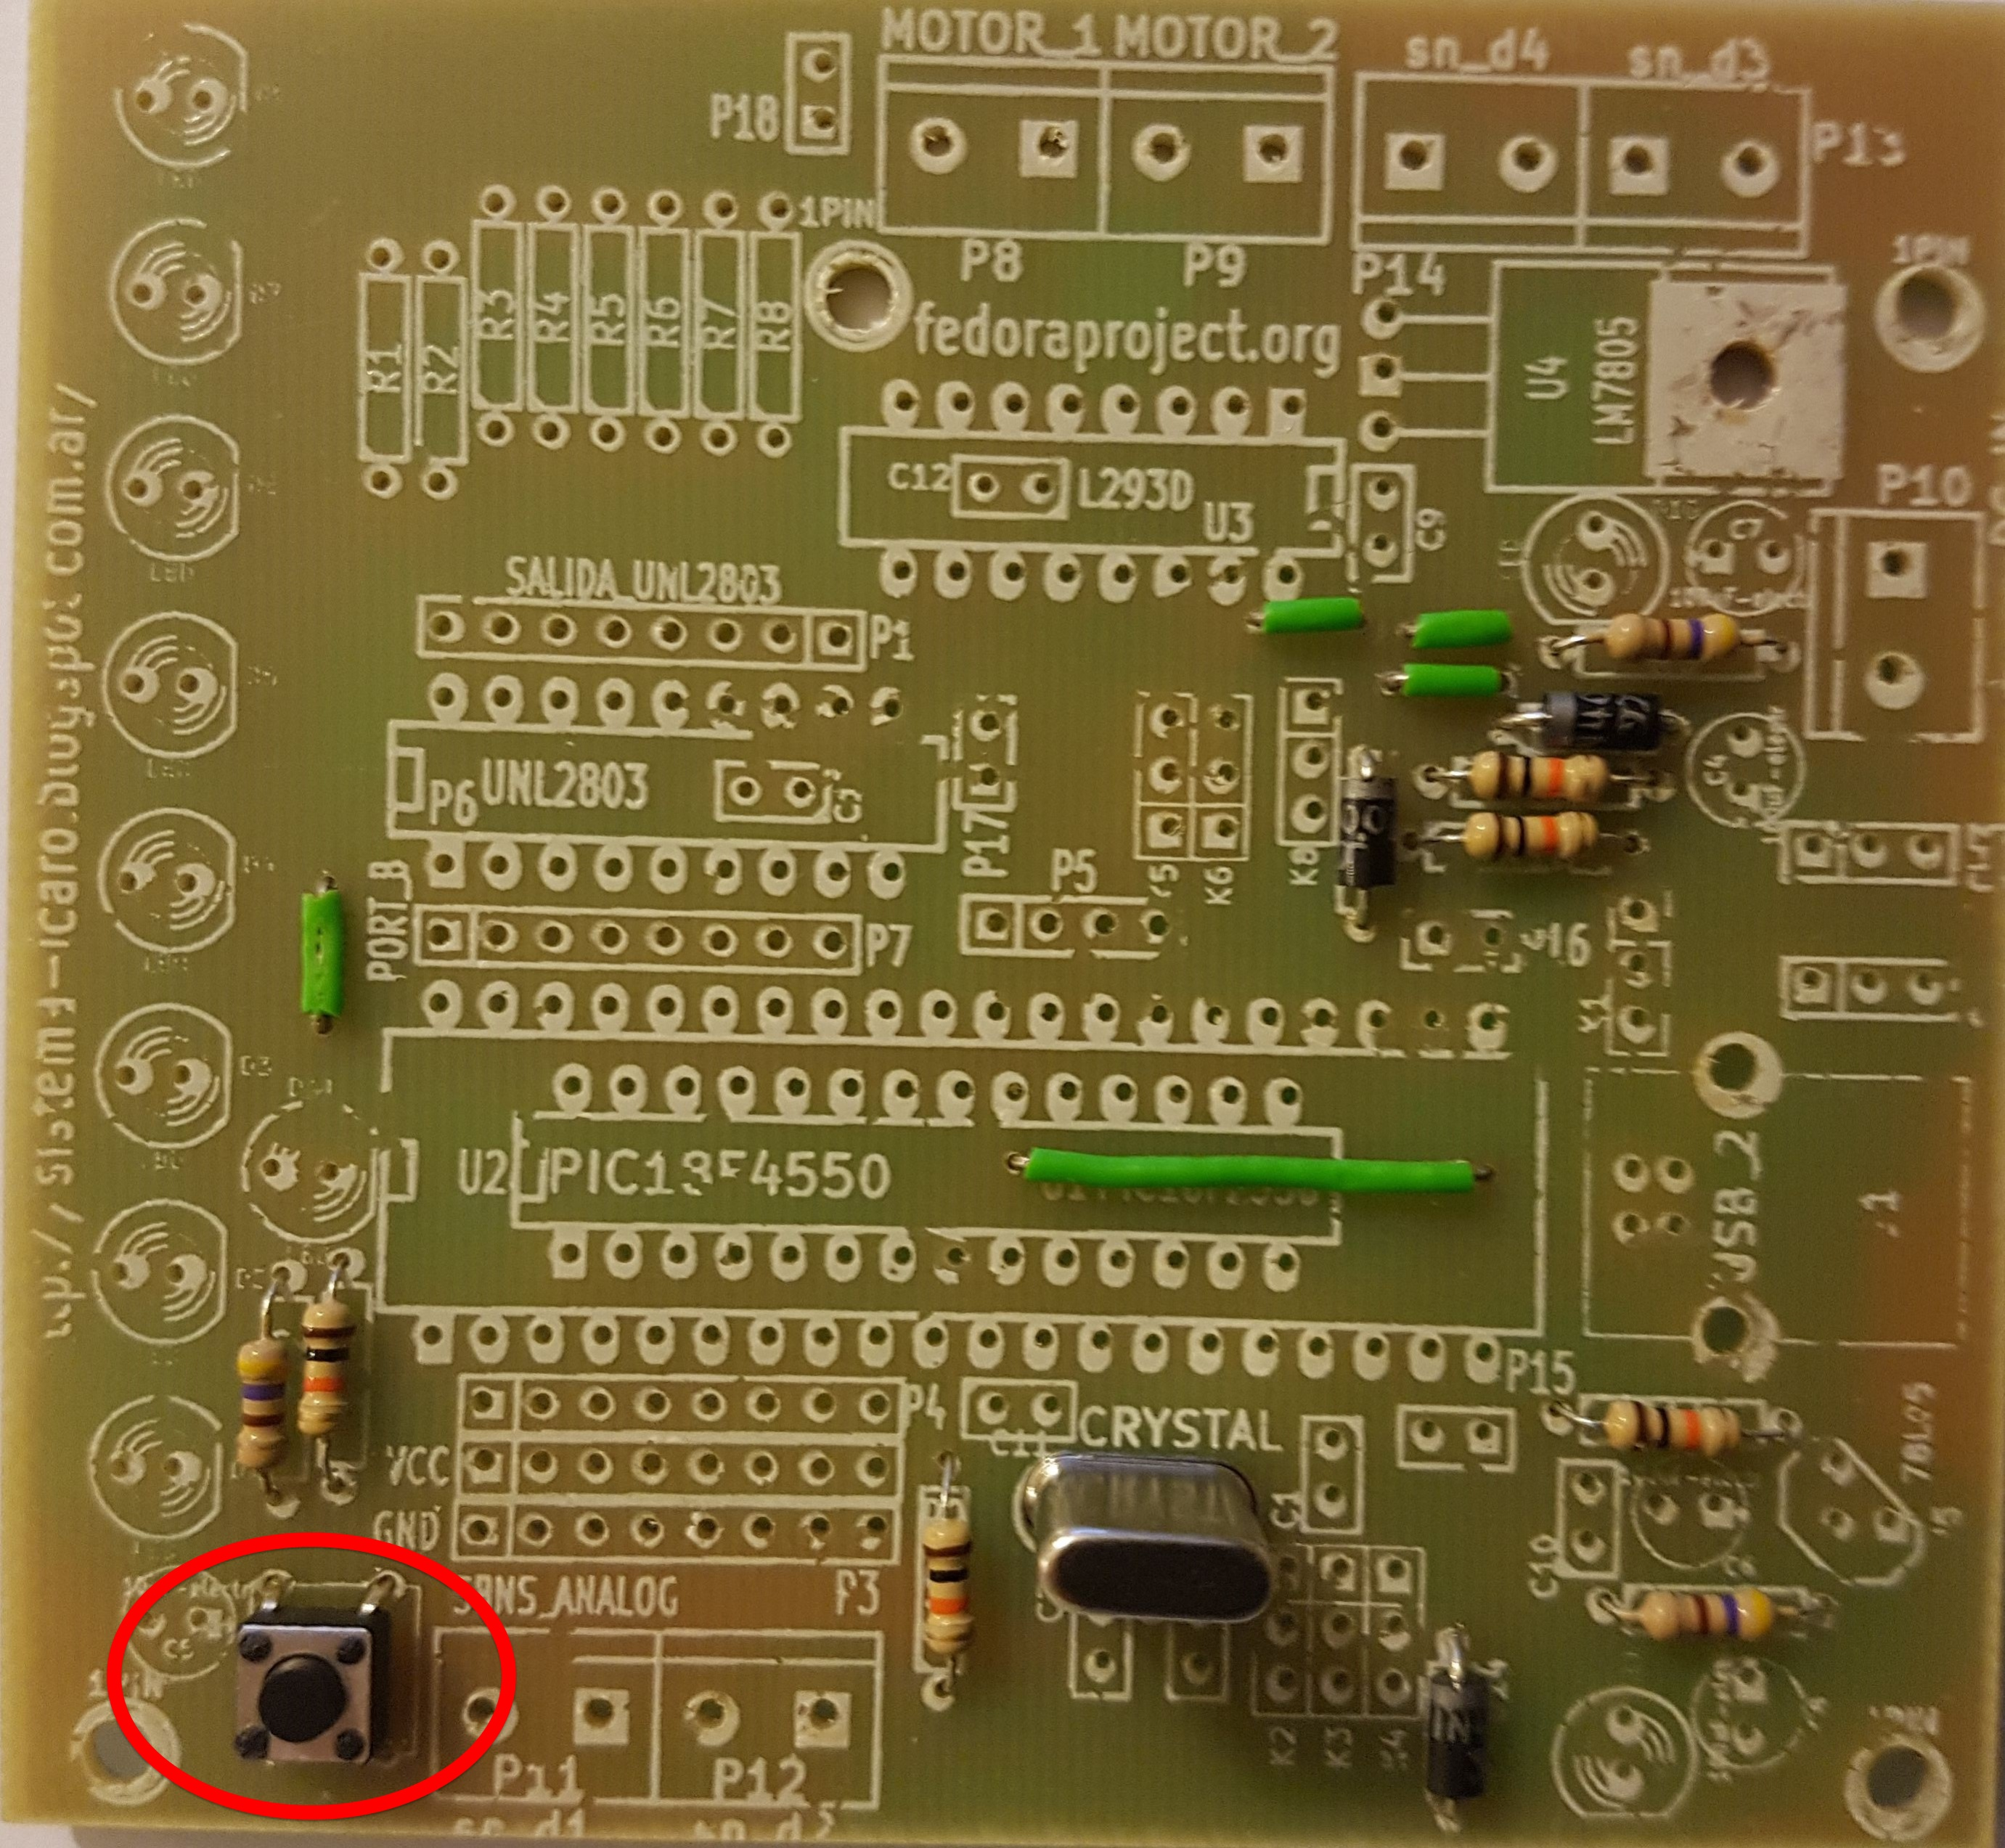
\includegraphics[width=0.8\linewidth]{Modulo_2/M2_2}
	\caption{Módulo 2 - Paso 2}
	\label{fig:M2_2}
\end{figure}

\newpage

\section{Paso 3:}

Instalar capacitor cerámico 220nF C1 

\begin{figure}[h]
	\centering
	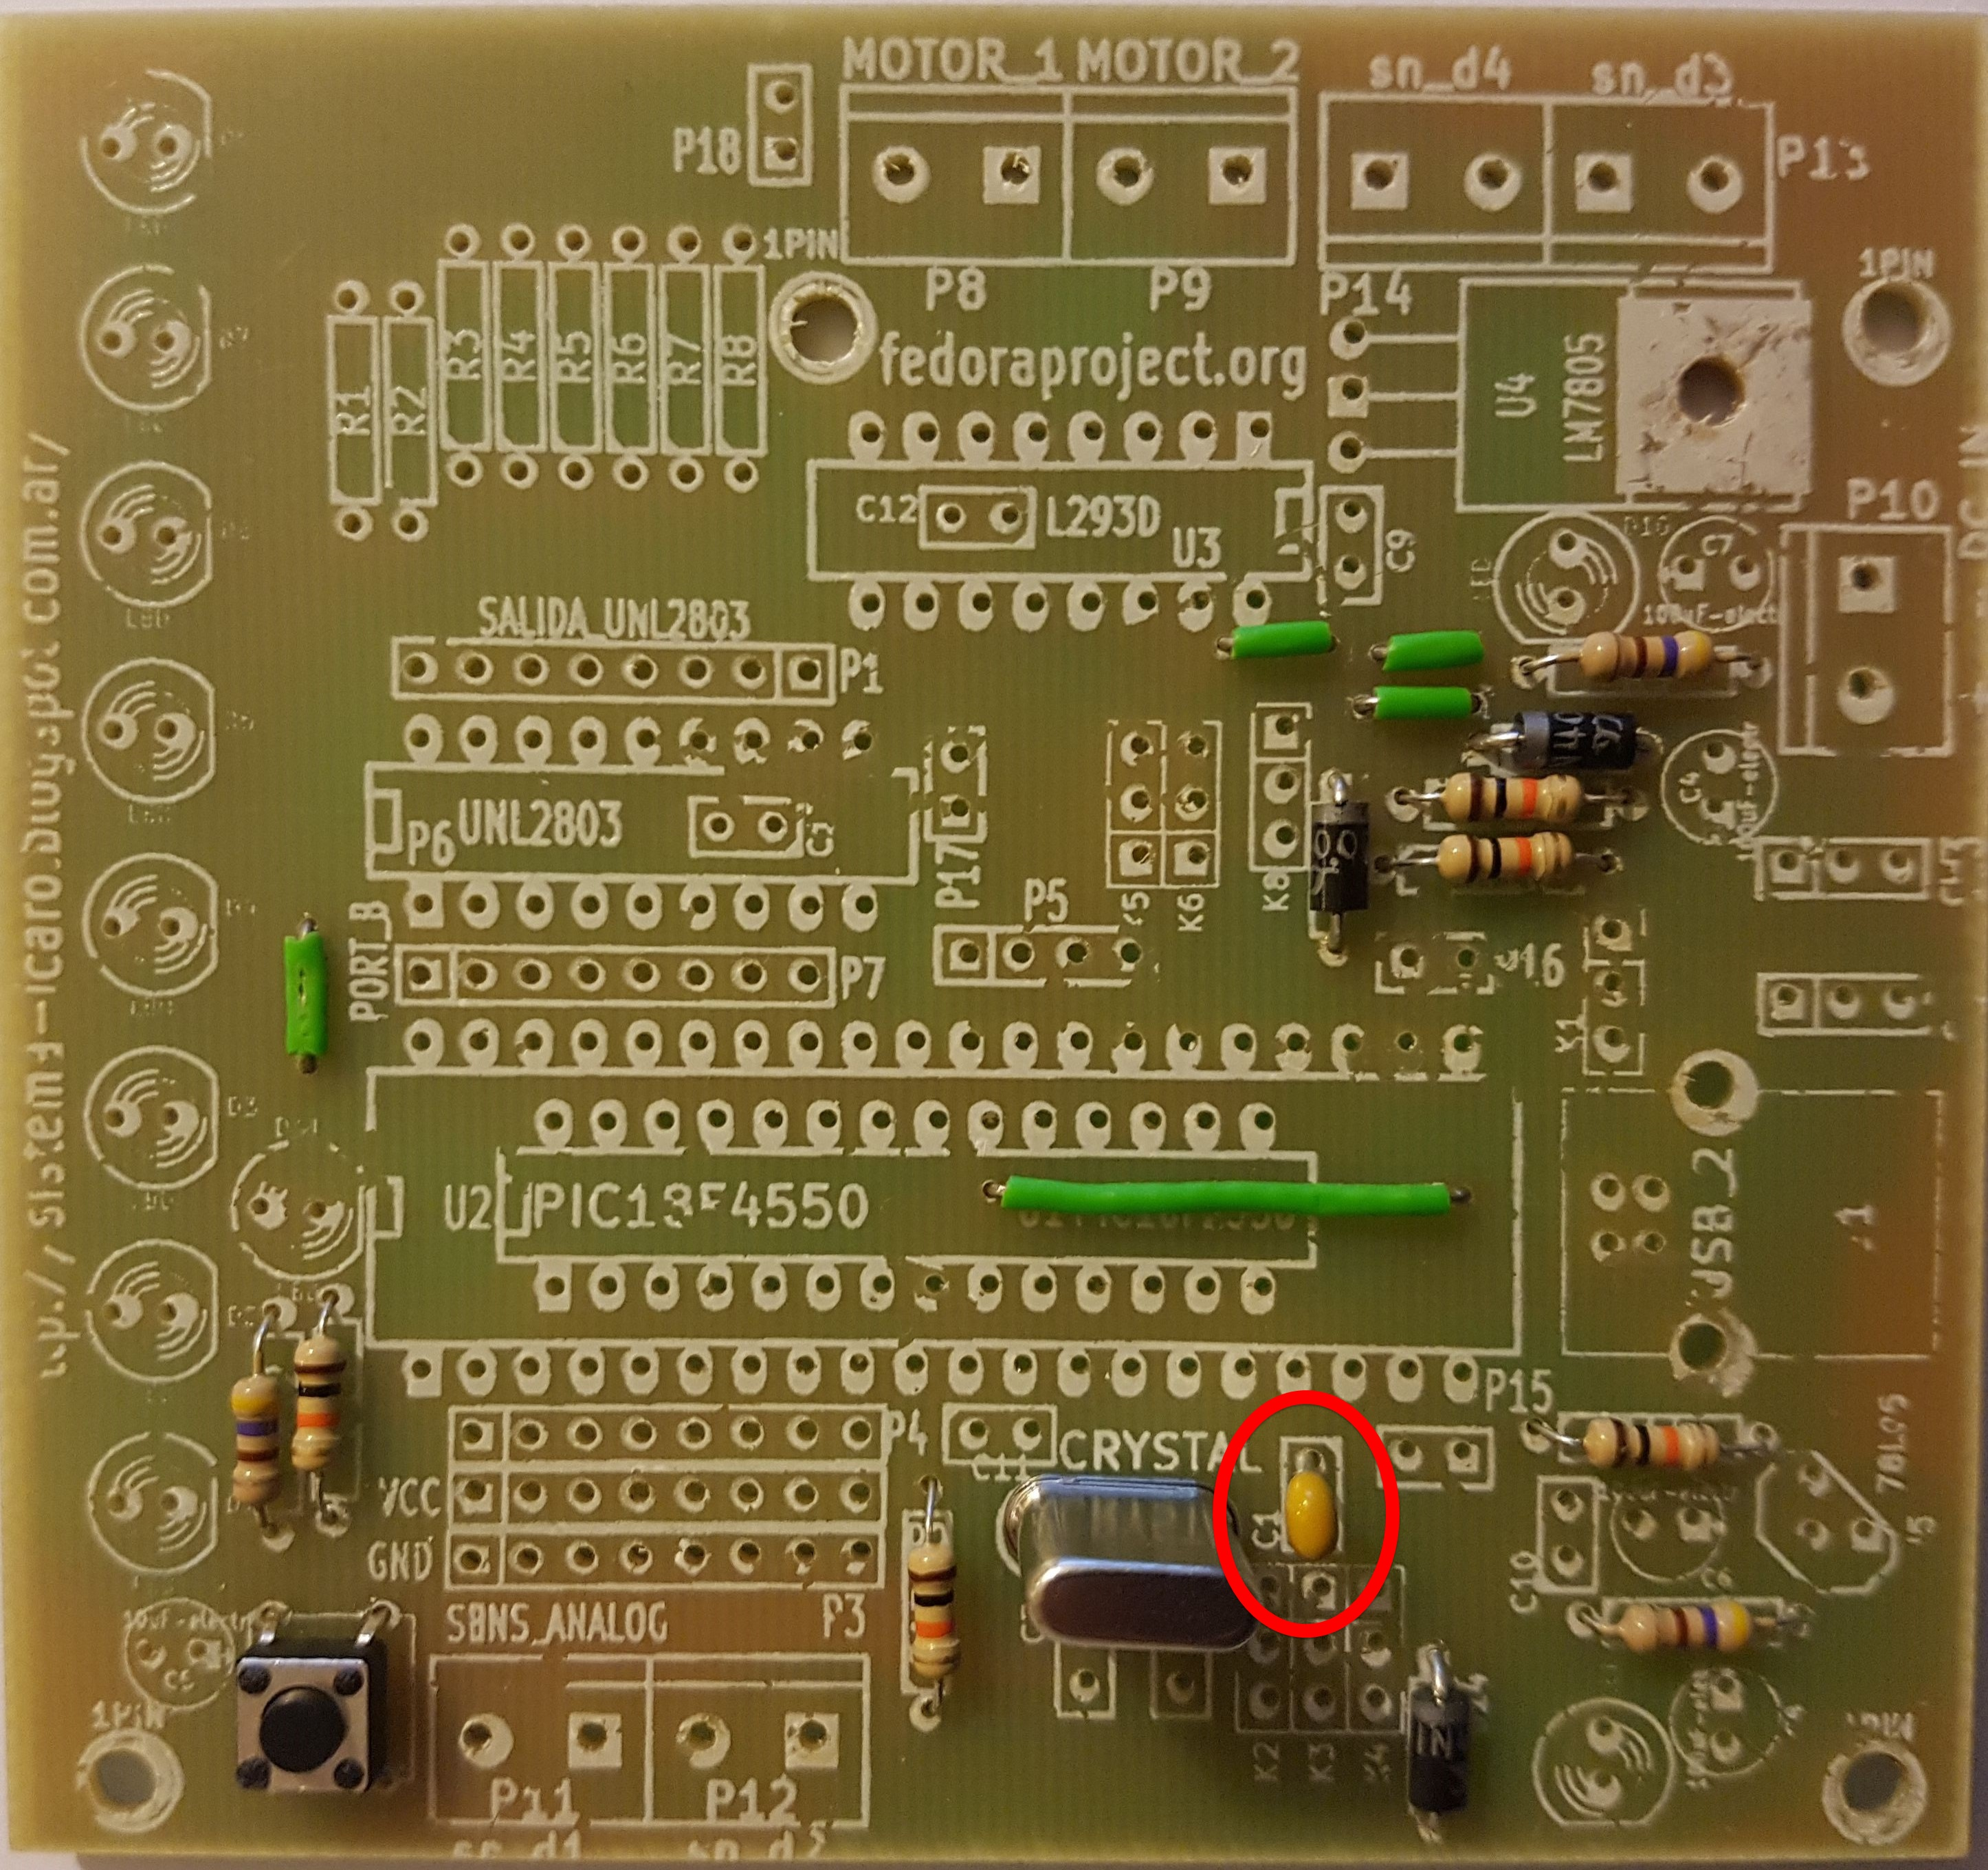
\includegraphics[width=0.8\linewidth]{Modulo_2/M2_3}
	\caption{Módulo 2 - Paso 3}
	\label{fig:M2_3}
\end{figure}

\newpage

\section{Paso 4:}

Instalar capacitor cerámico 0.1uF C11

\begin{figure}[h]
	\centering
	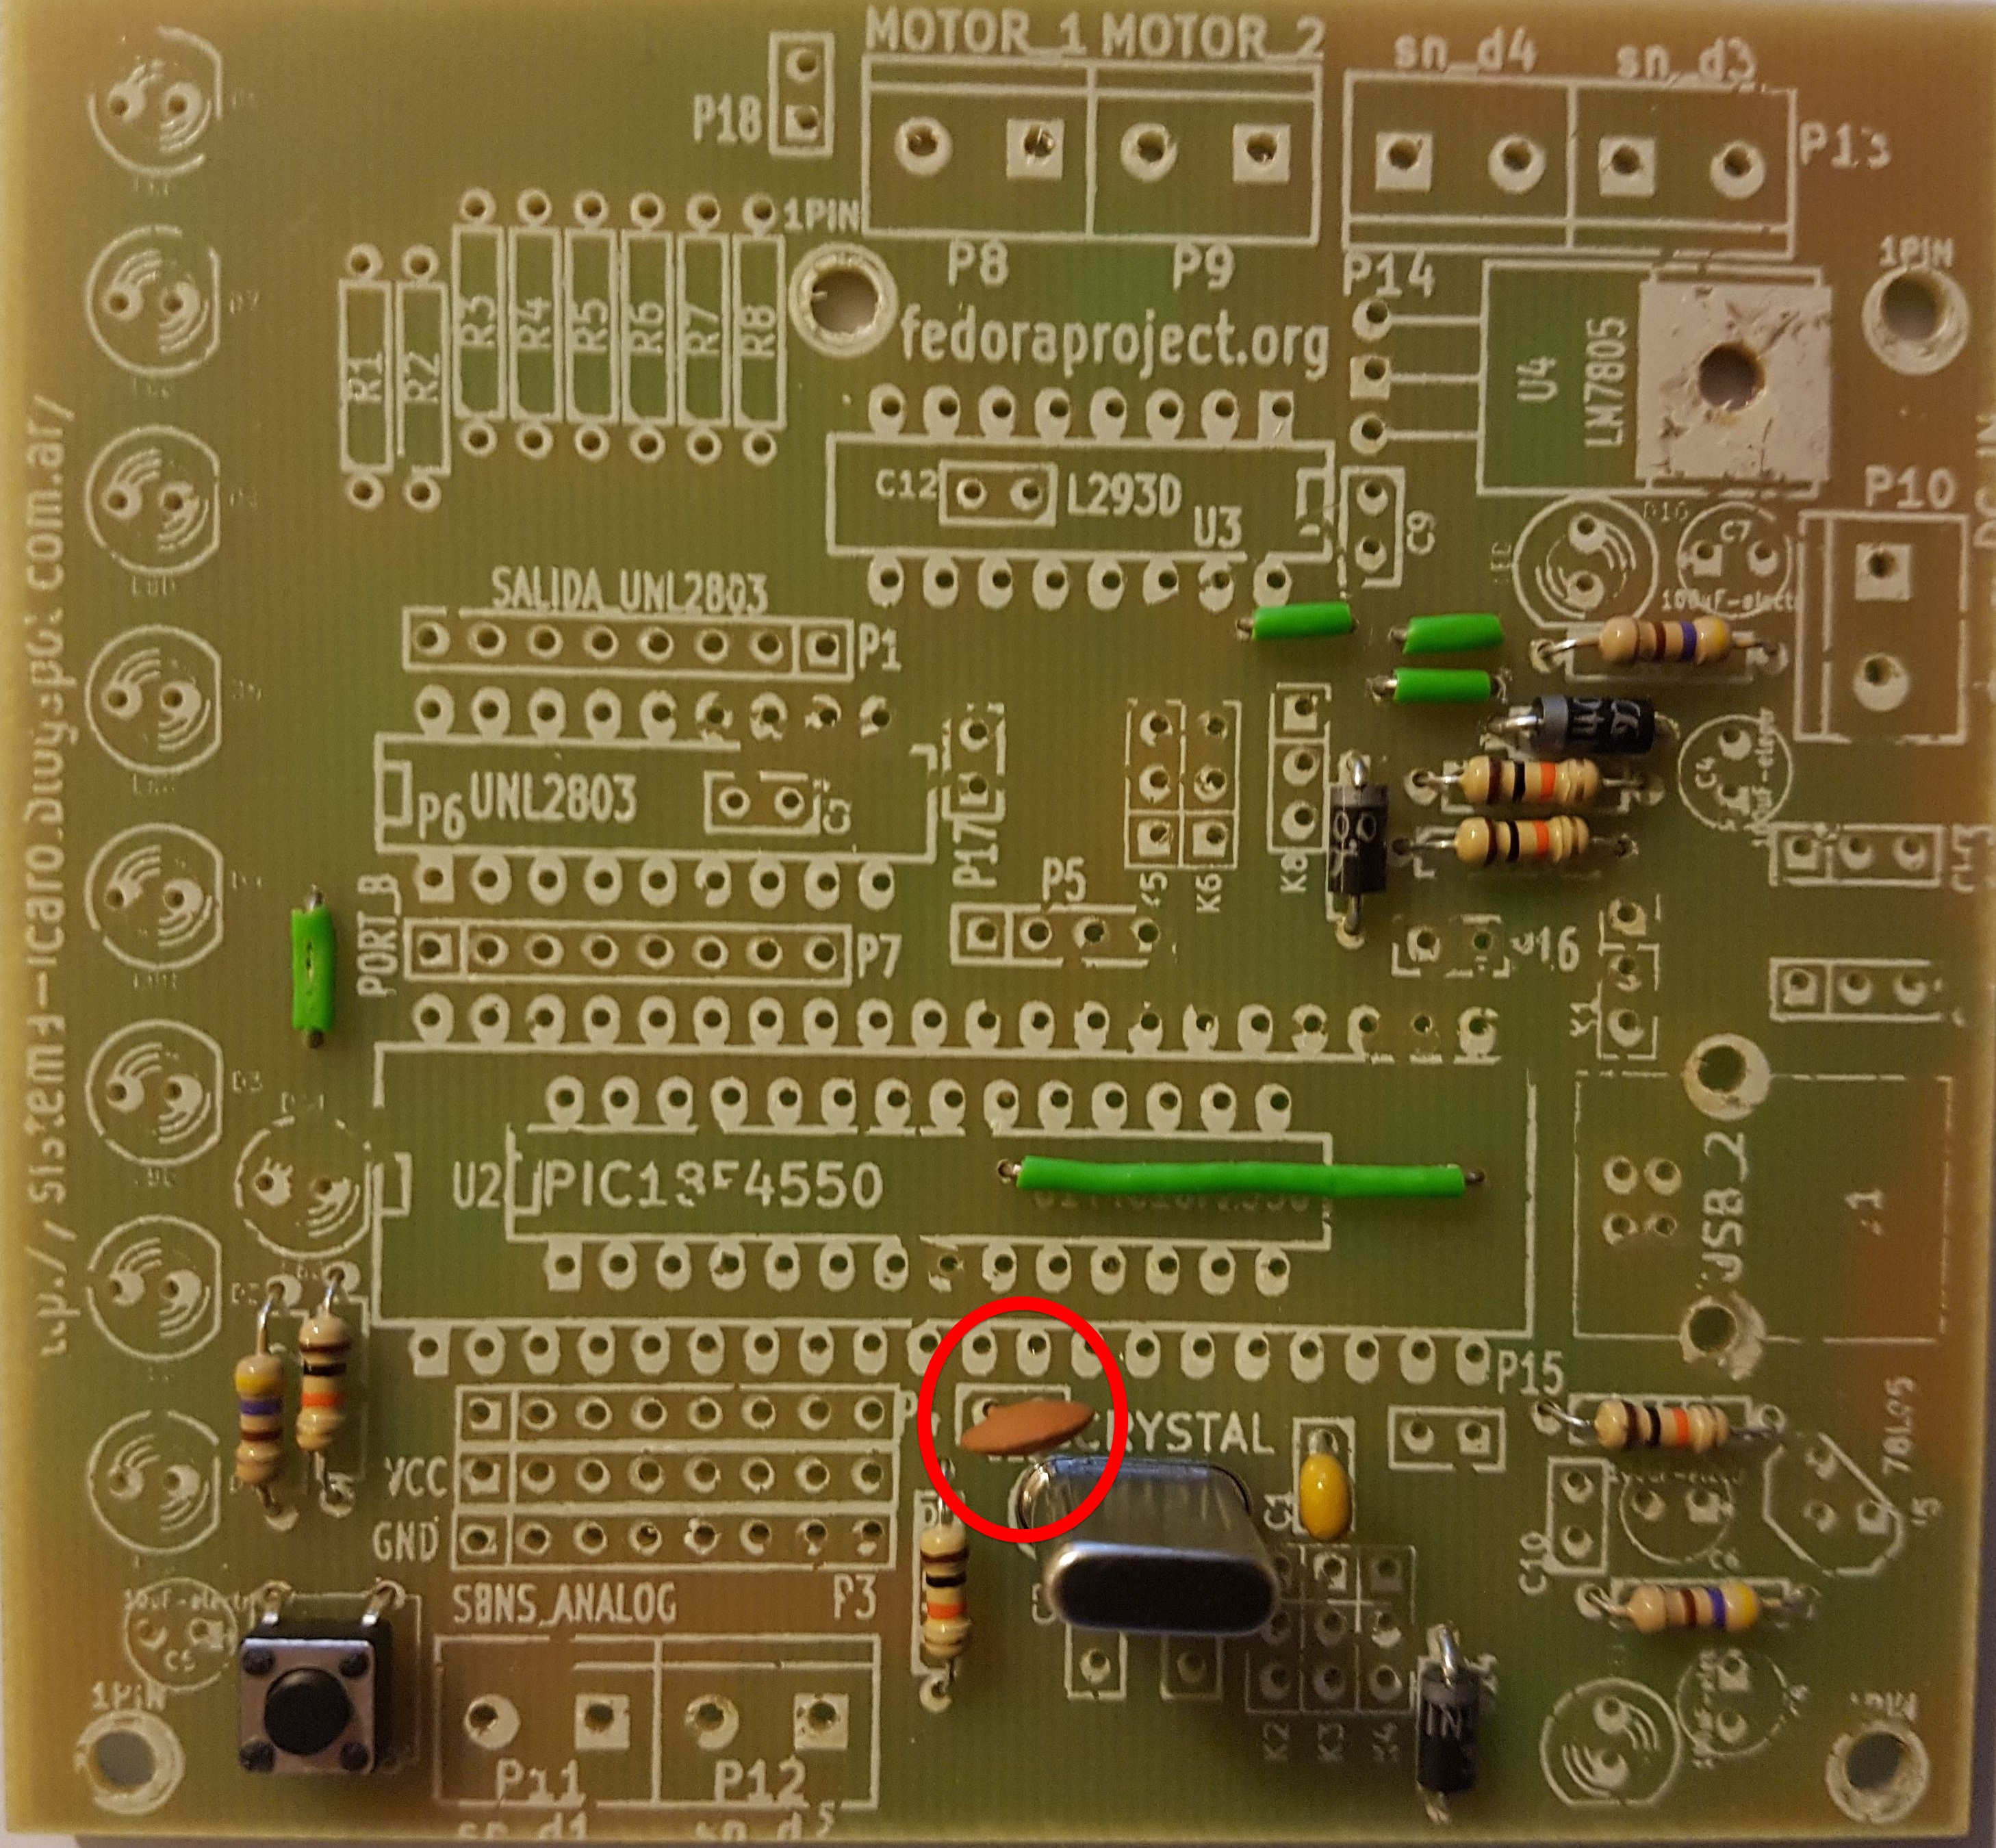
\includegraphics[width=0.8\linewidth]{Modulo_2/M2_4}
	\caption{Módulo 2 - Paso 4}
	\label{fig:M2_4}
\end{figure}

\newpage

\section{Paso 5:}

Instalar capacitadores cerámicos 22pF C2 y C3

\begin{figure}[h]
	\centering
	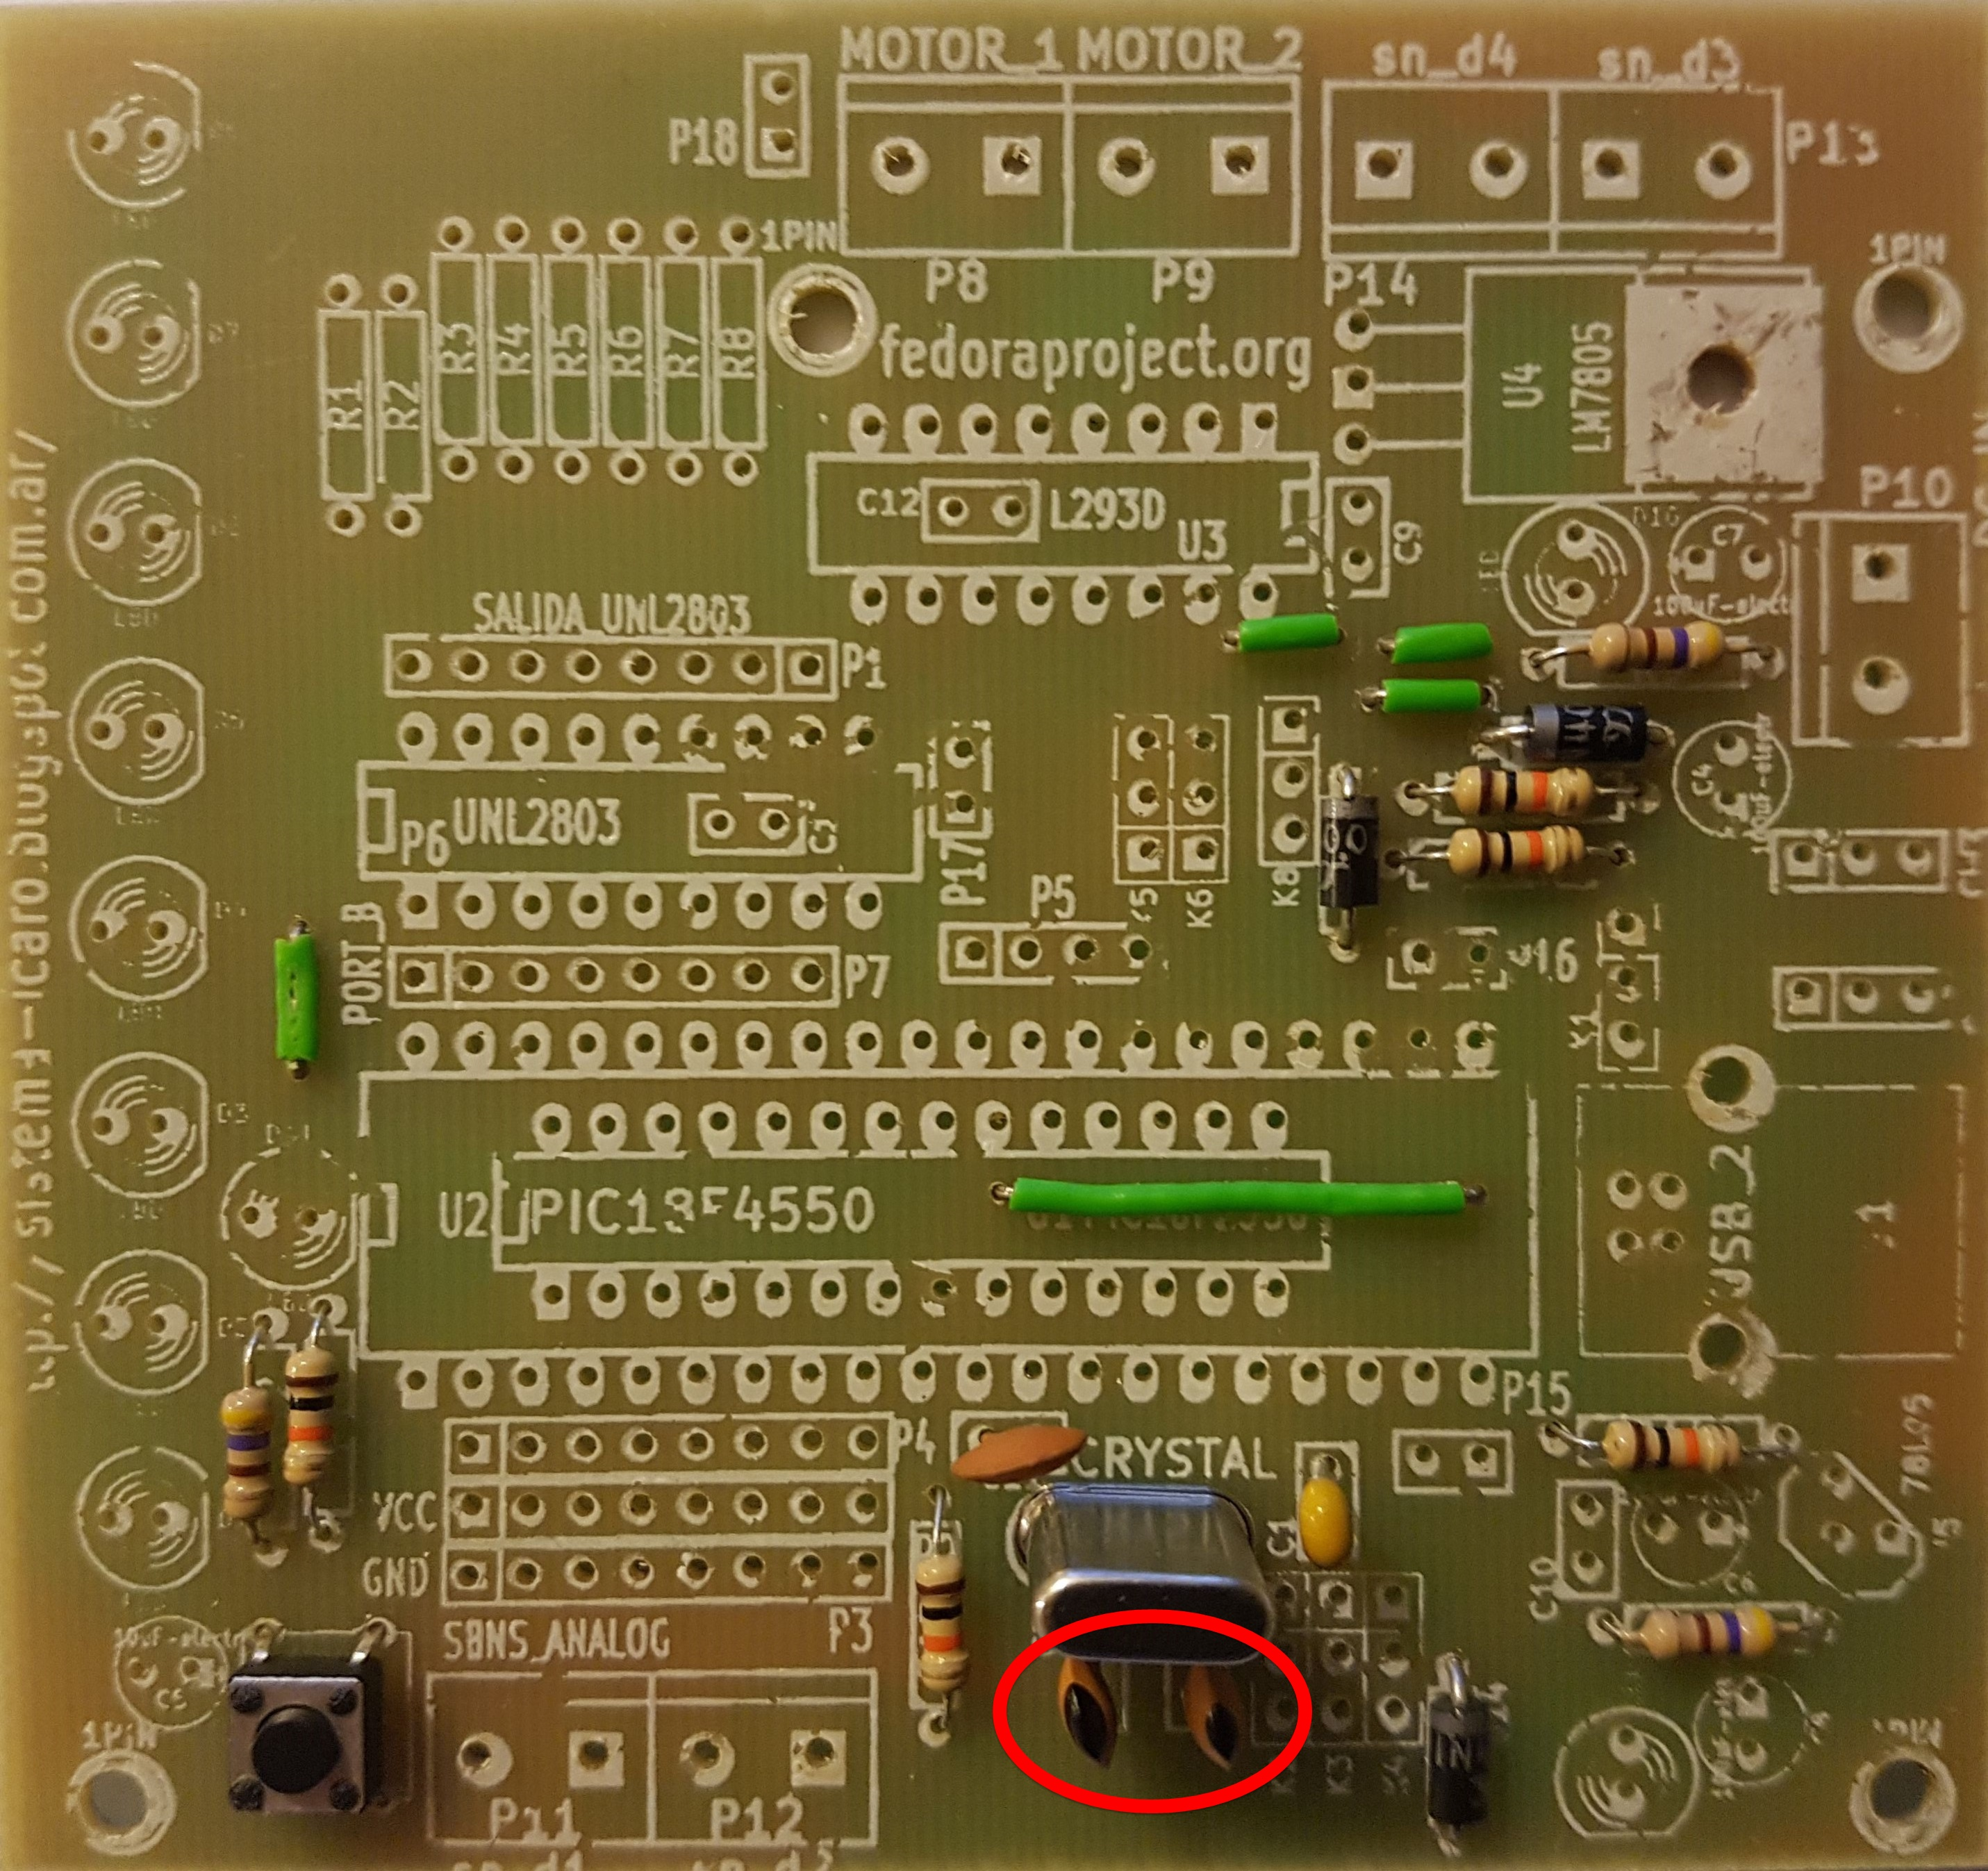
\includegraphics[width=0.8\linewidth]{Modulo_2/M2_5}
	\caption{Módulo 2 - Paso 5}
	\label{fig:M2_5}
\end{figure}

\newpage

\section{Paso 6:}

Instalar Sócalo de 40 patas (20x2) U2 Tomar en cuenta alinear la muesca del diagrama de la placa con la muesca del zócalo.

\begin{figure}[h]
	\centering
	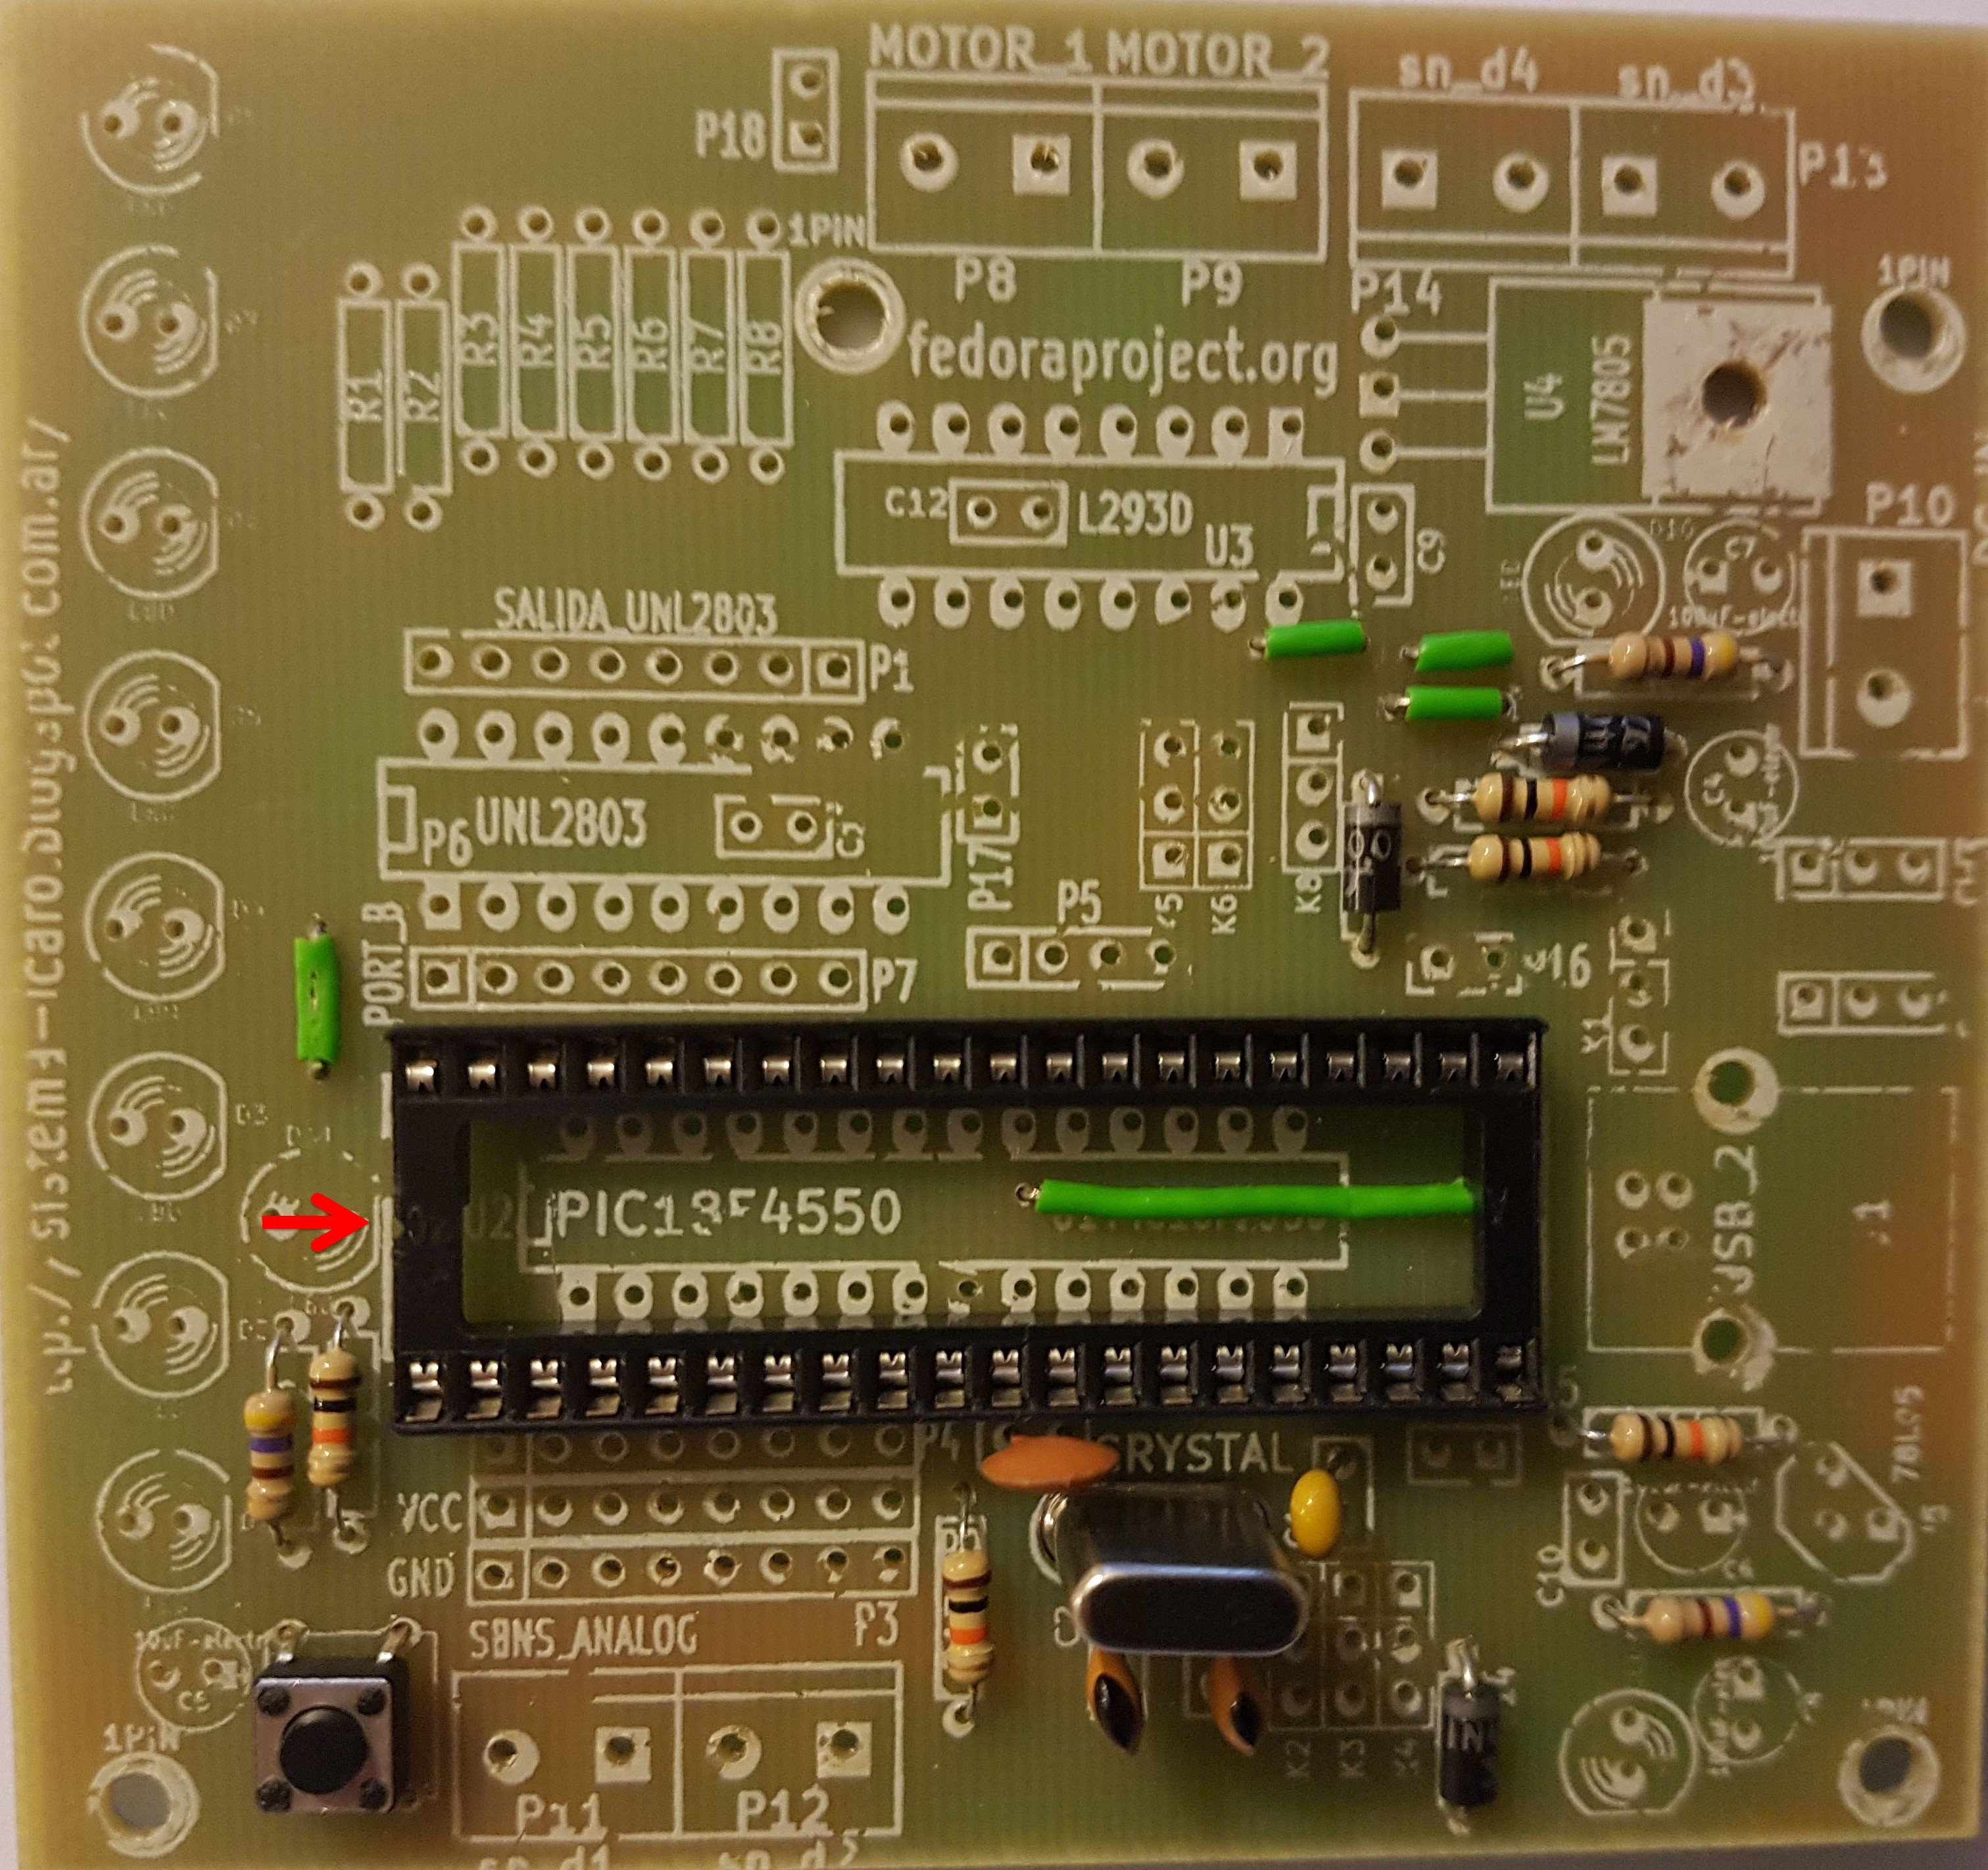
\includegraphics[width=0.8\linewidth]{Modulo_2/M2_6}
	\caption{Módulo 2 - Paso 6}
	\label{fig:M2_6}
\end{figure}

\newpage

\section{Paso 7:}

Instalar led del microcontrolador. D11 (Se recomienda color rojo)

\begin{figure}[h]
	\centering
	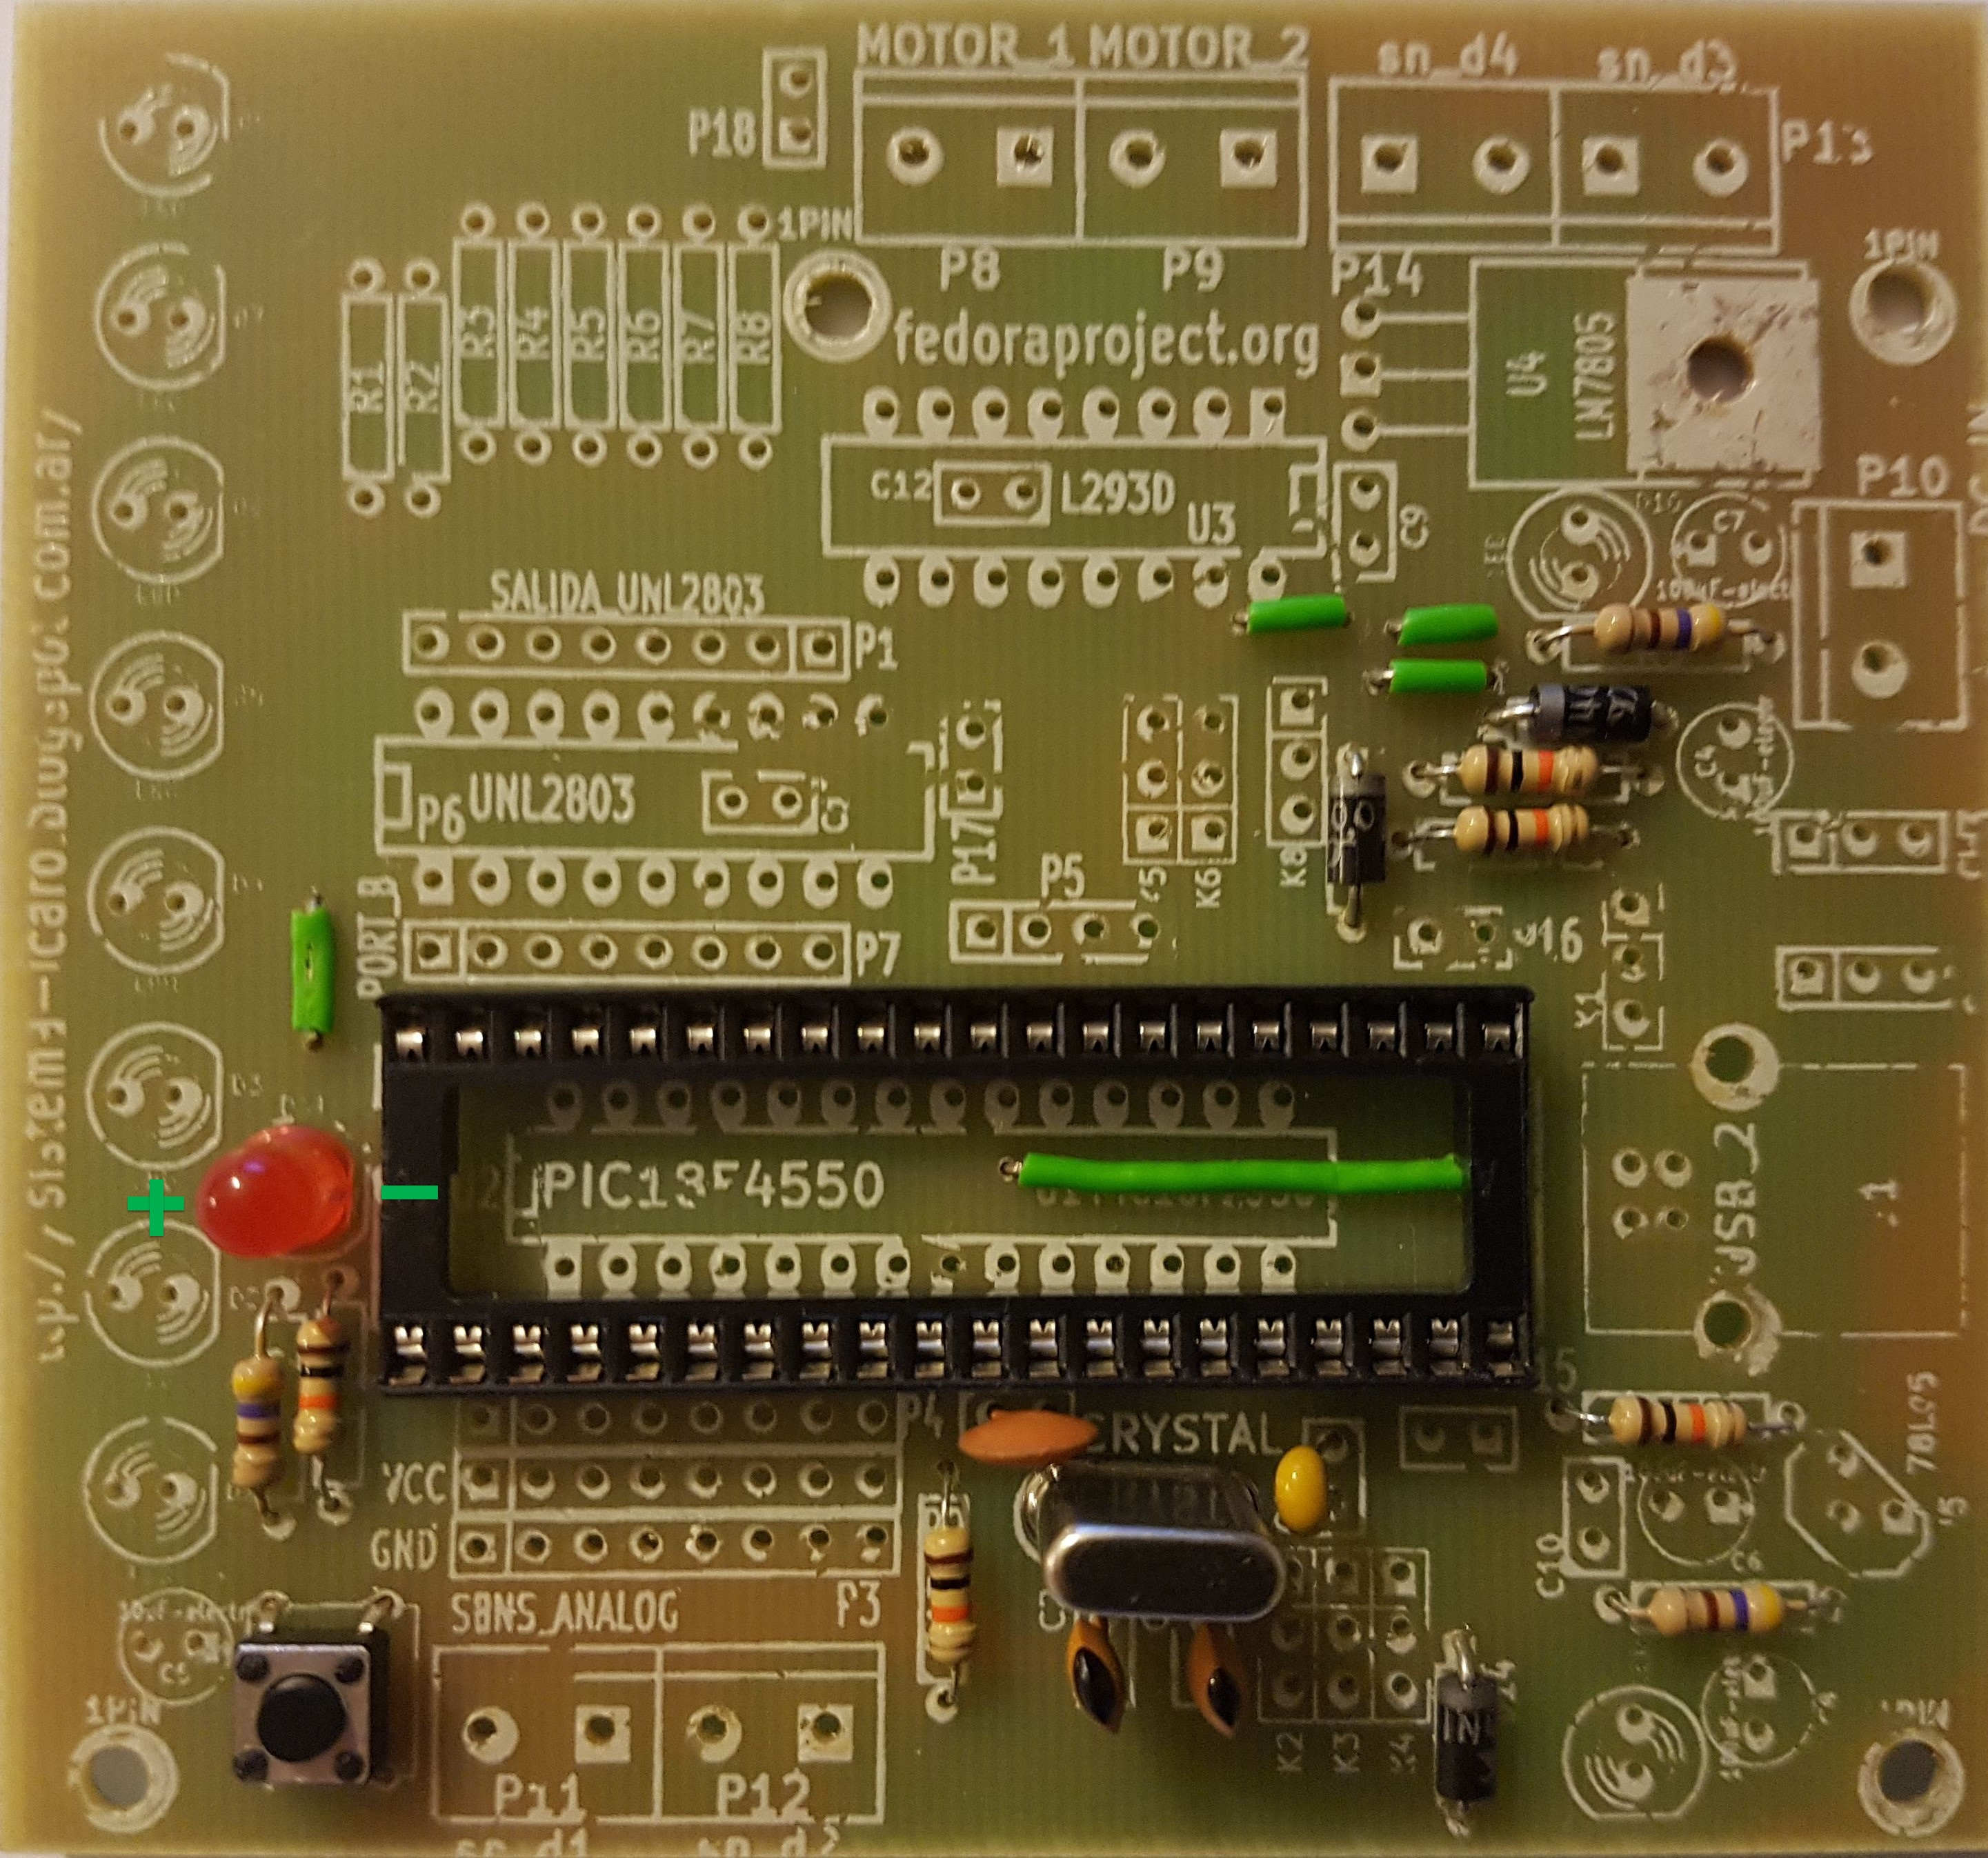
\includegraphics[width=0.8\linewidth]{Modulo_2/M2_7}
	\caption{Módulo 2 - Paso 7}
	\label{fig:M2_7}
\end{figure}

\newpage

\section{Paso 8:}

Instalar pines machos K1

\begin{figure}[h]
	\centering
	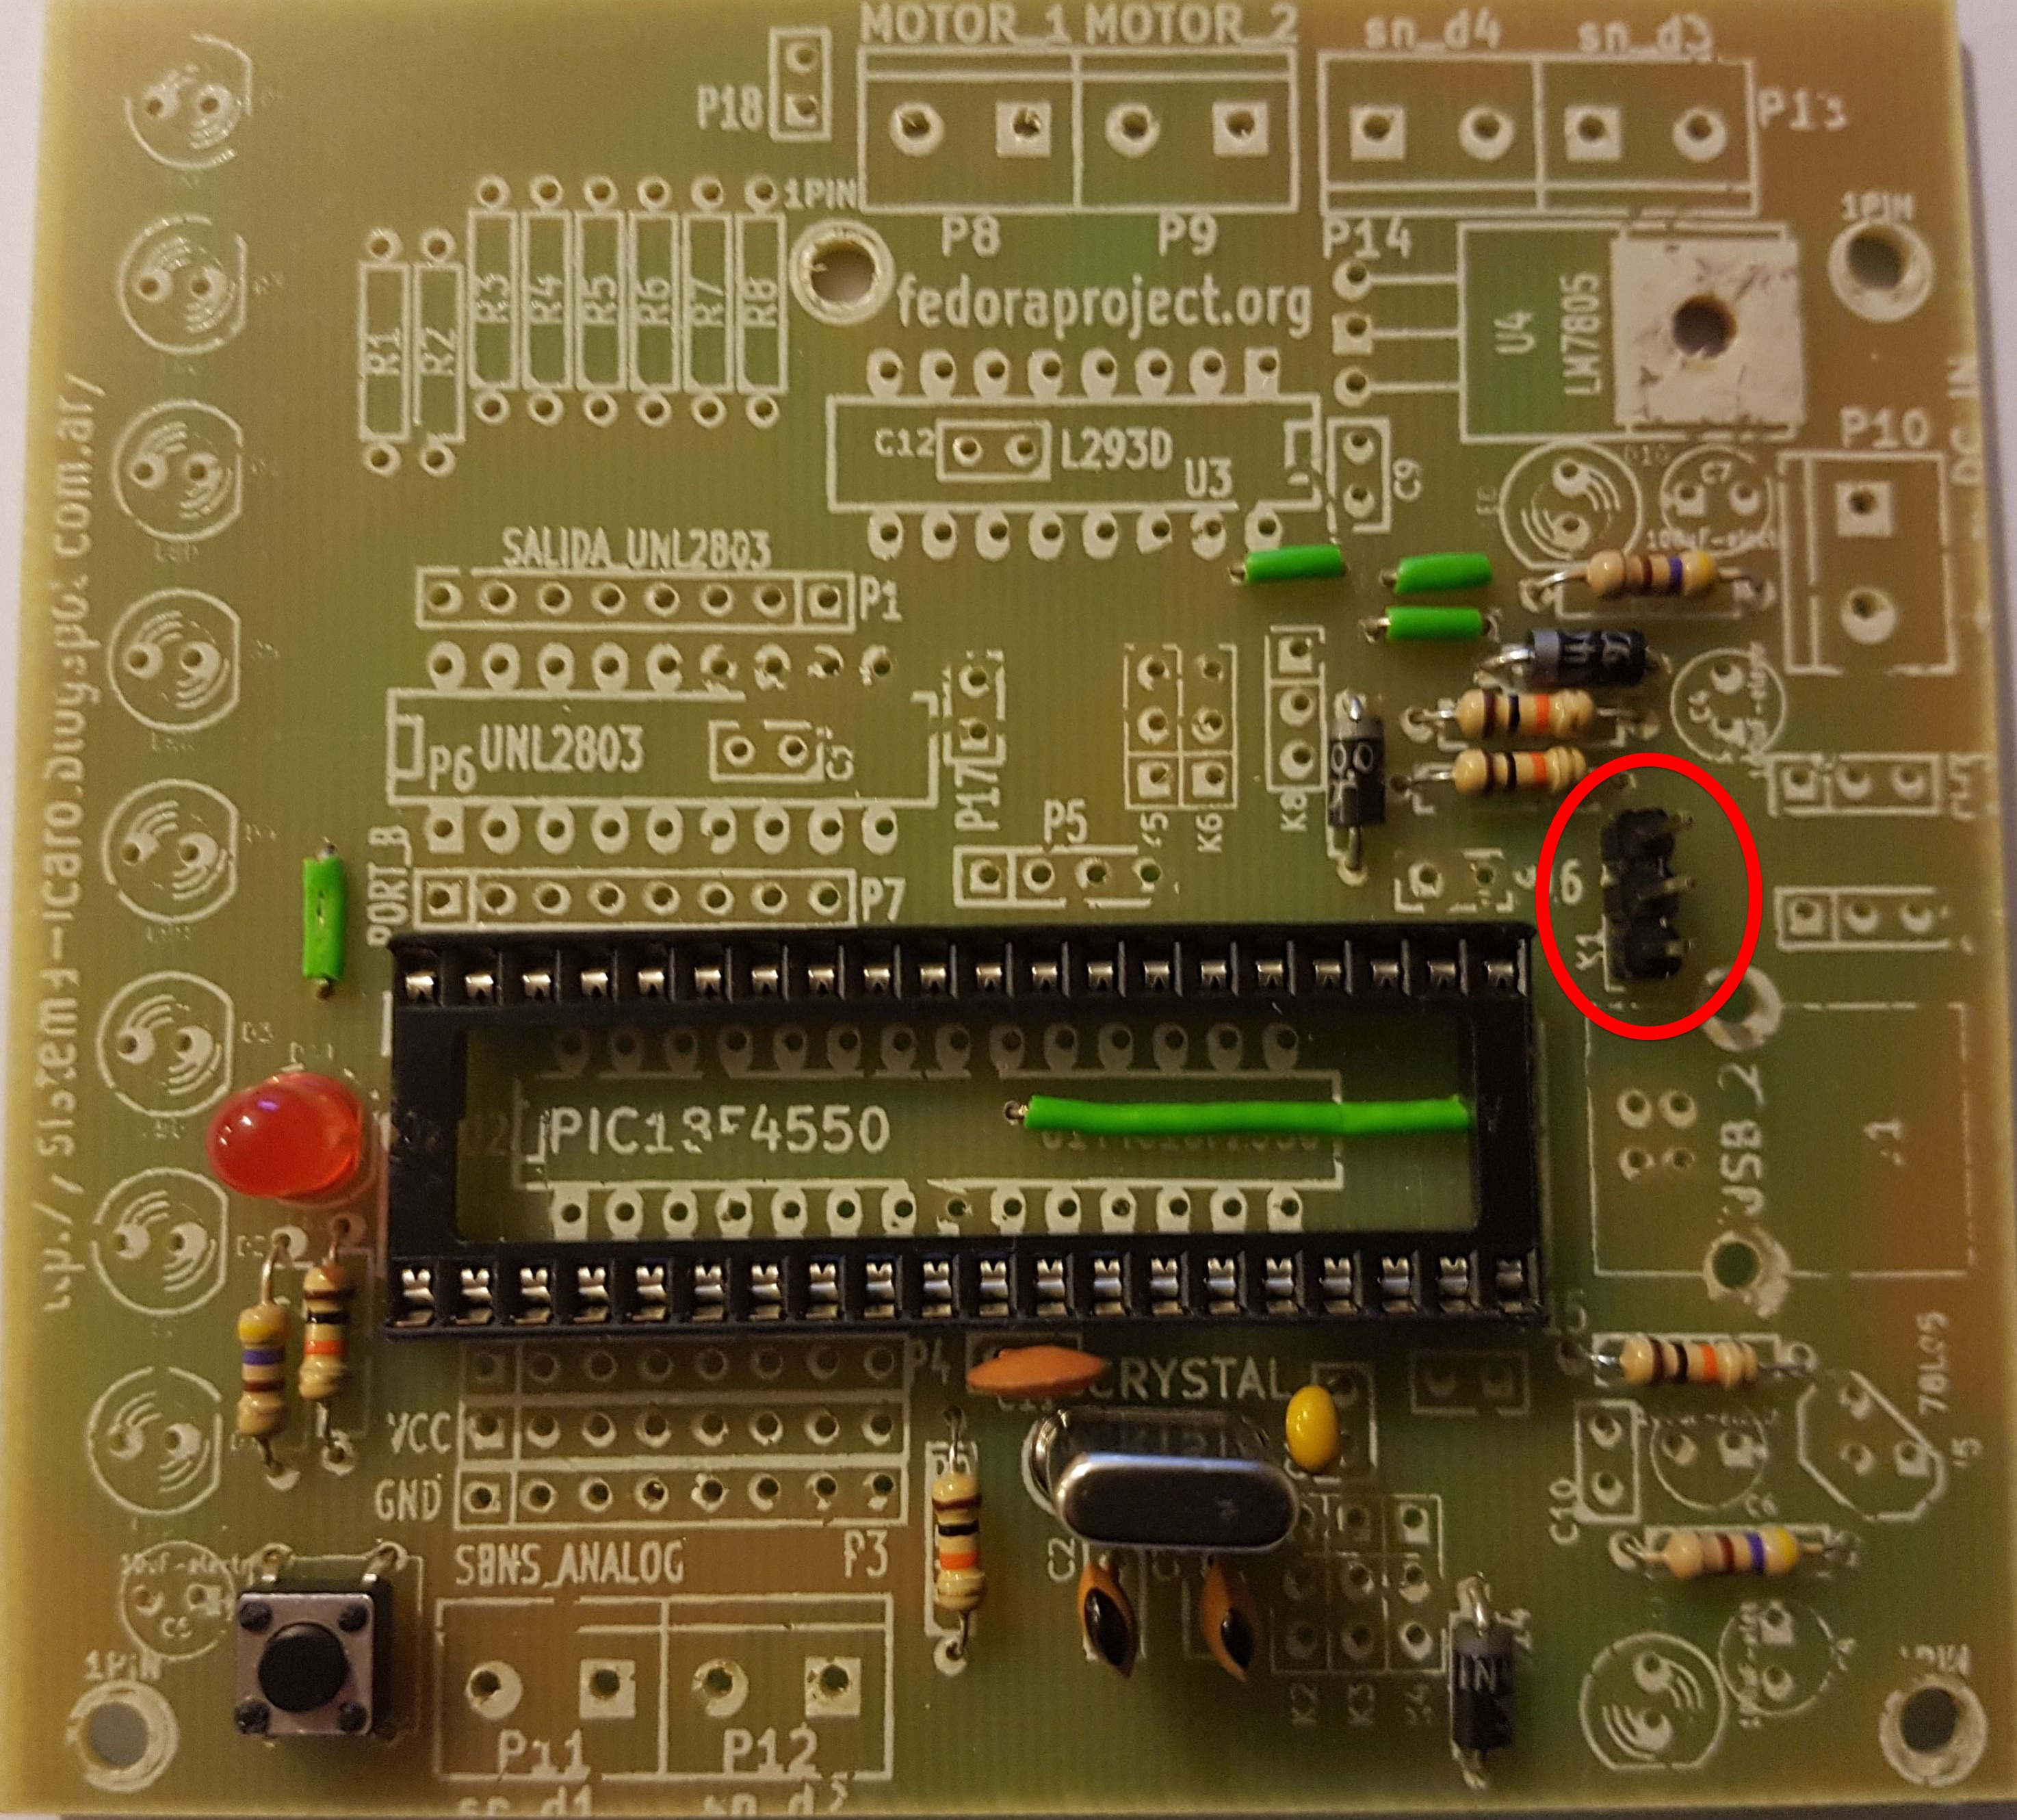
\includegraphics[width=0.8\linewidth]{Modulo_2/M2_8}
	\caption{Módulo 2 - Paso 8}
	\label{fig:M2_8}
\end{figure}

\newpage

\section{Paso 9:}

Instalar capacitor electrolítico 10uF. C5

\begin{figure}[h]
	\centering
	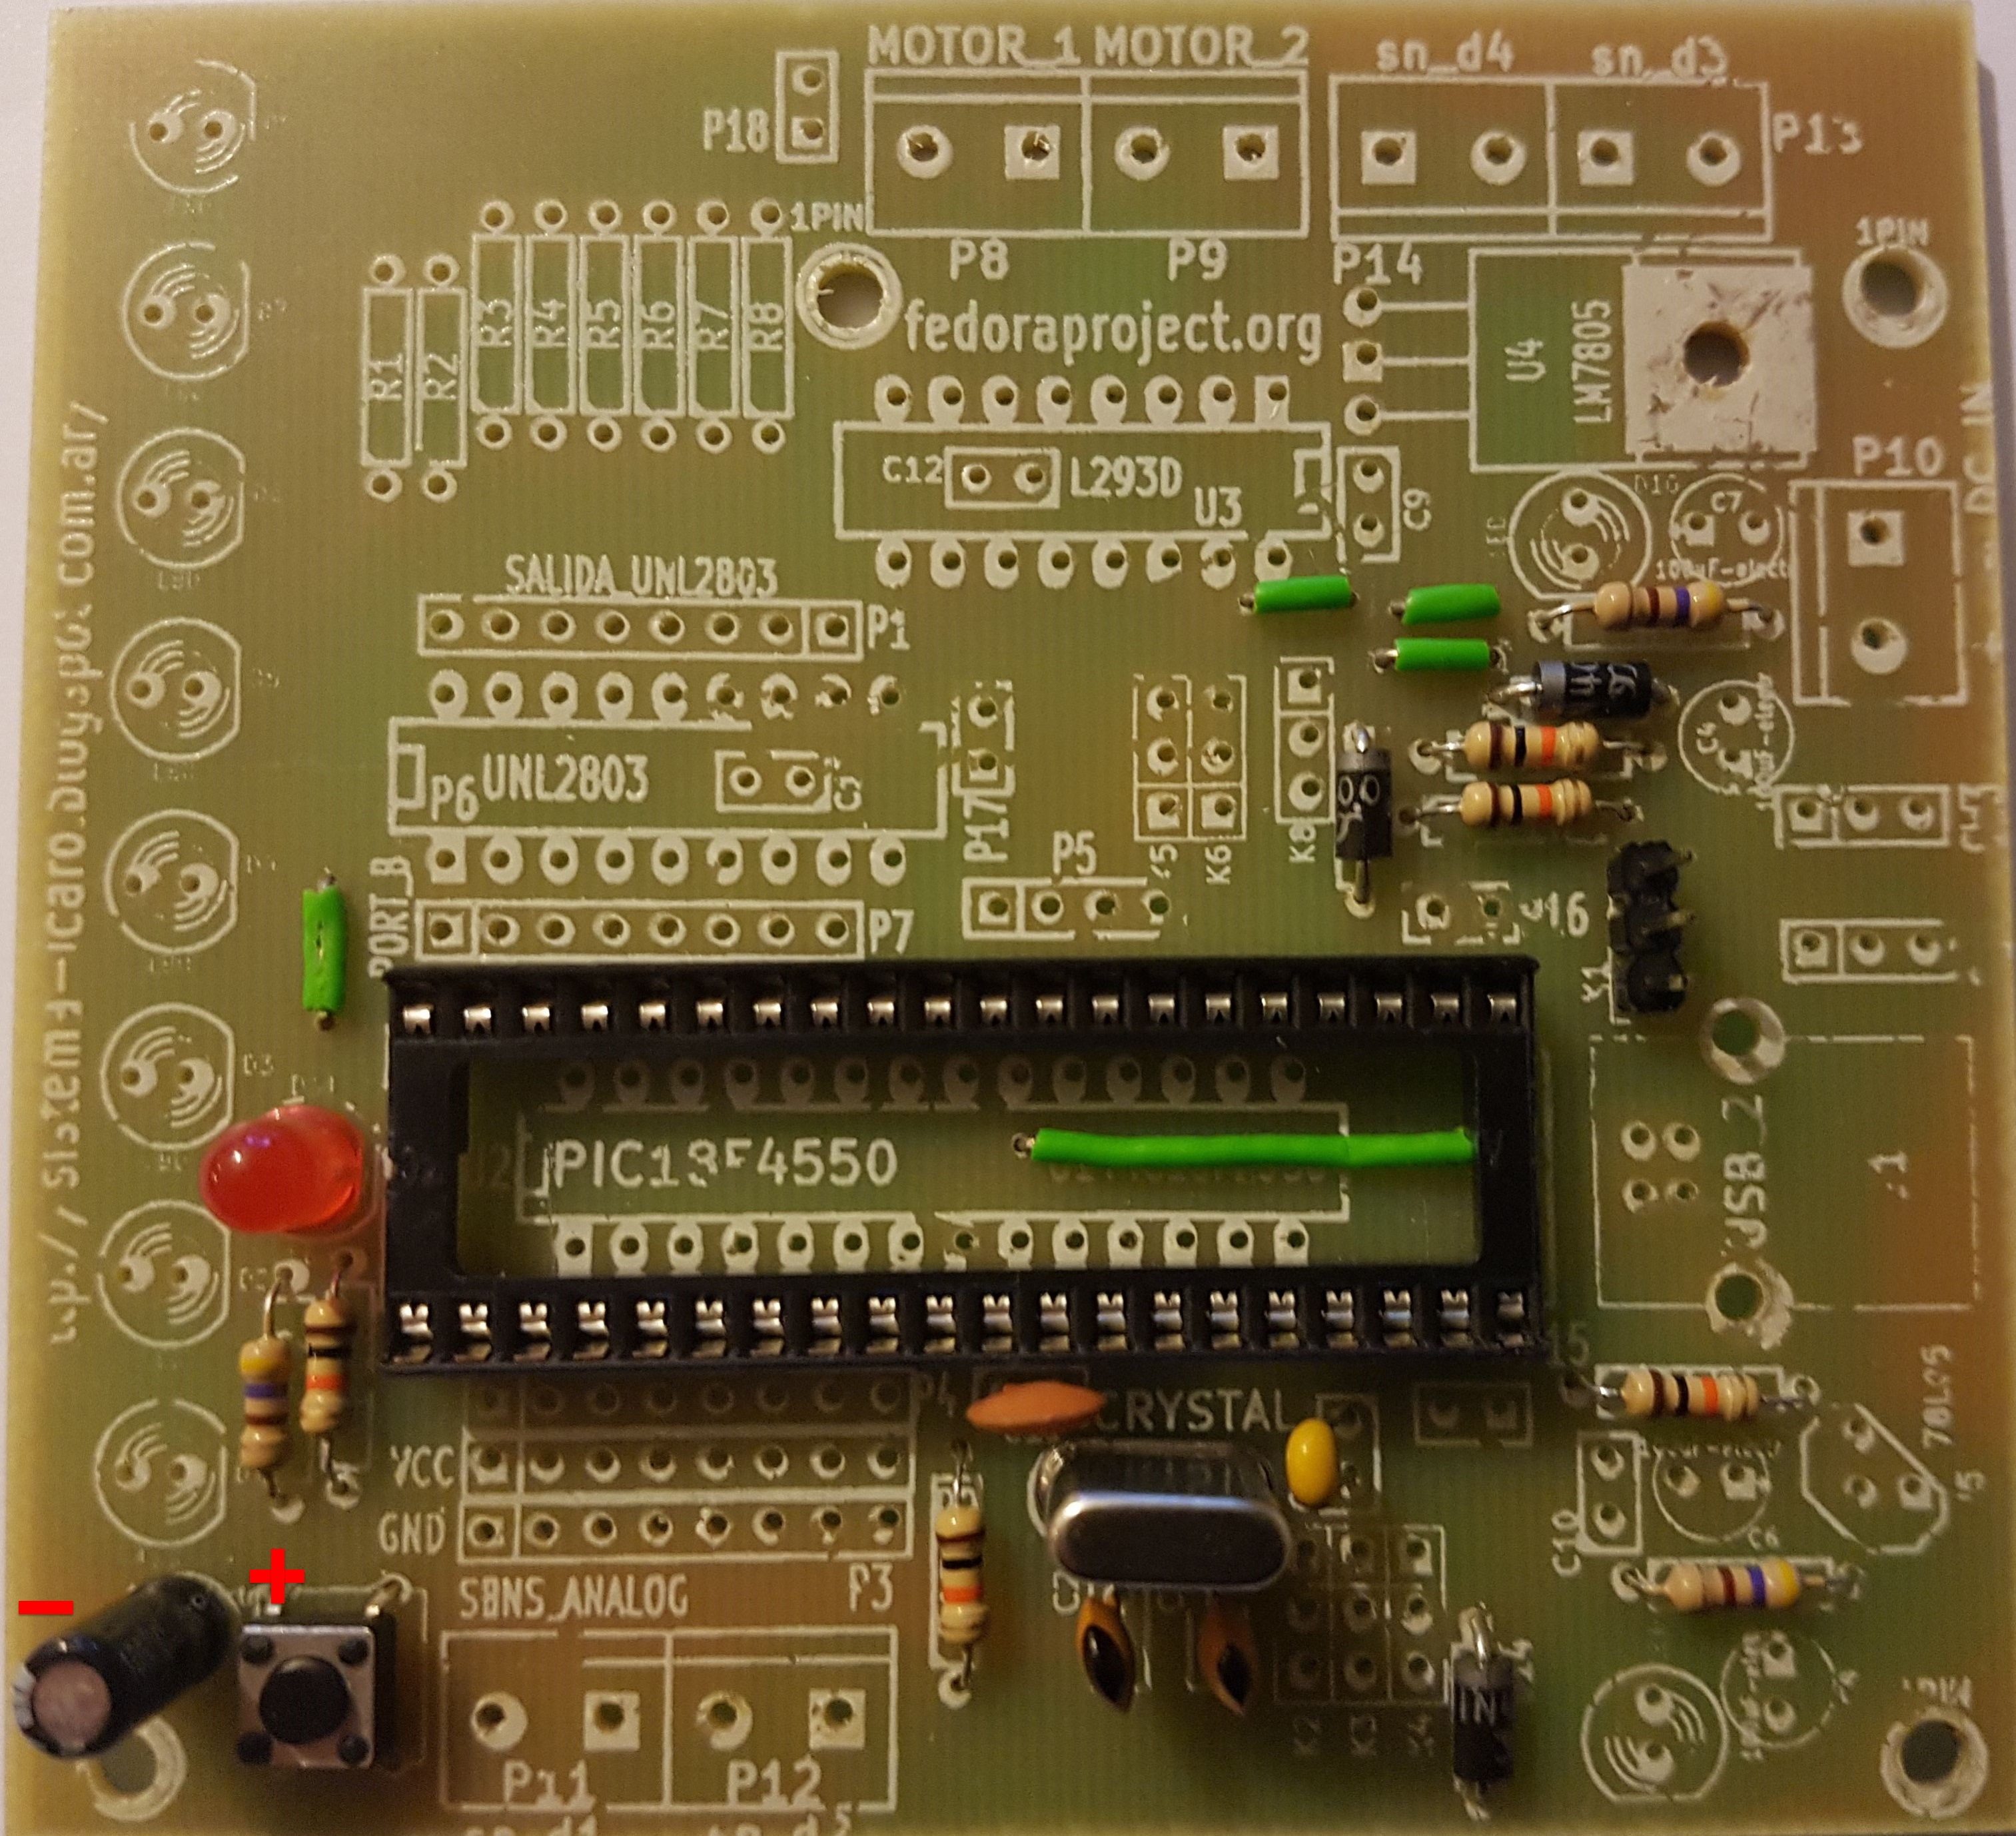
\includegraphics[width=0.8\linewidth]{Modulo_2/M2_9}
	\caption{Módulo 2 - Paso 9}
	\label{fig:M2_9}
\end{figure}

\newpage

\section{Paso 10:}

Instalar puerto USB. J1

\begin{figure}[h]
	\centering
	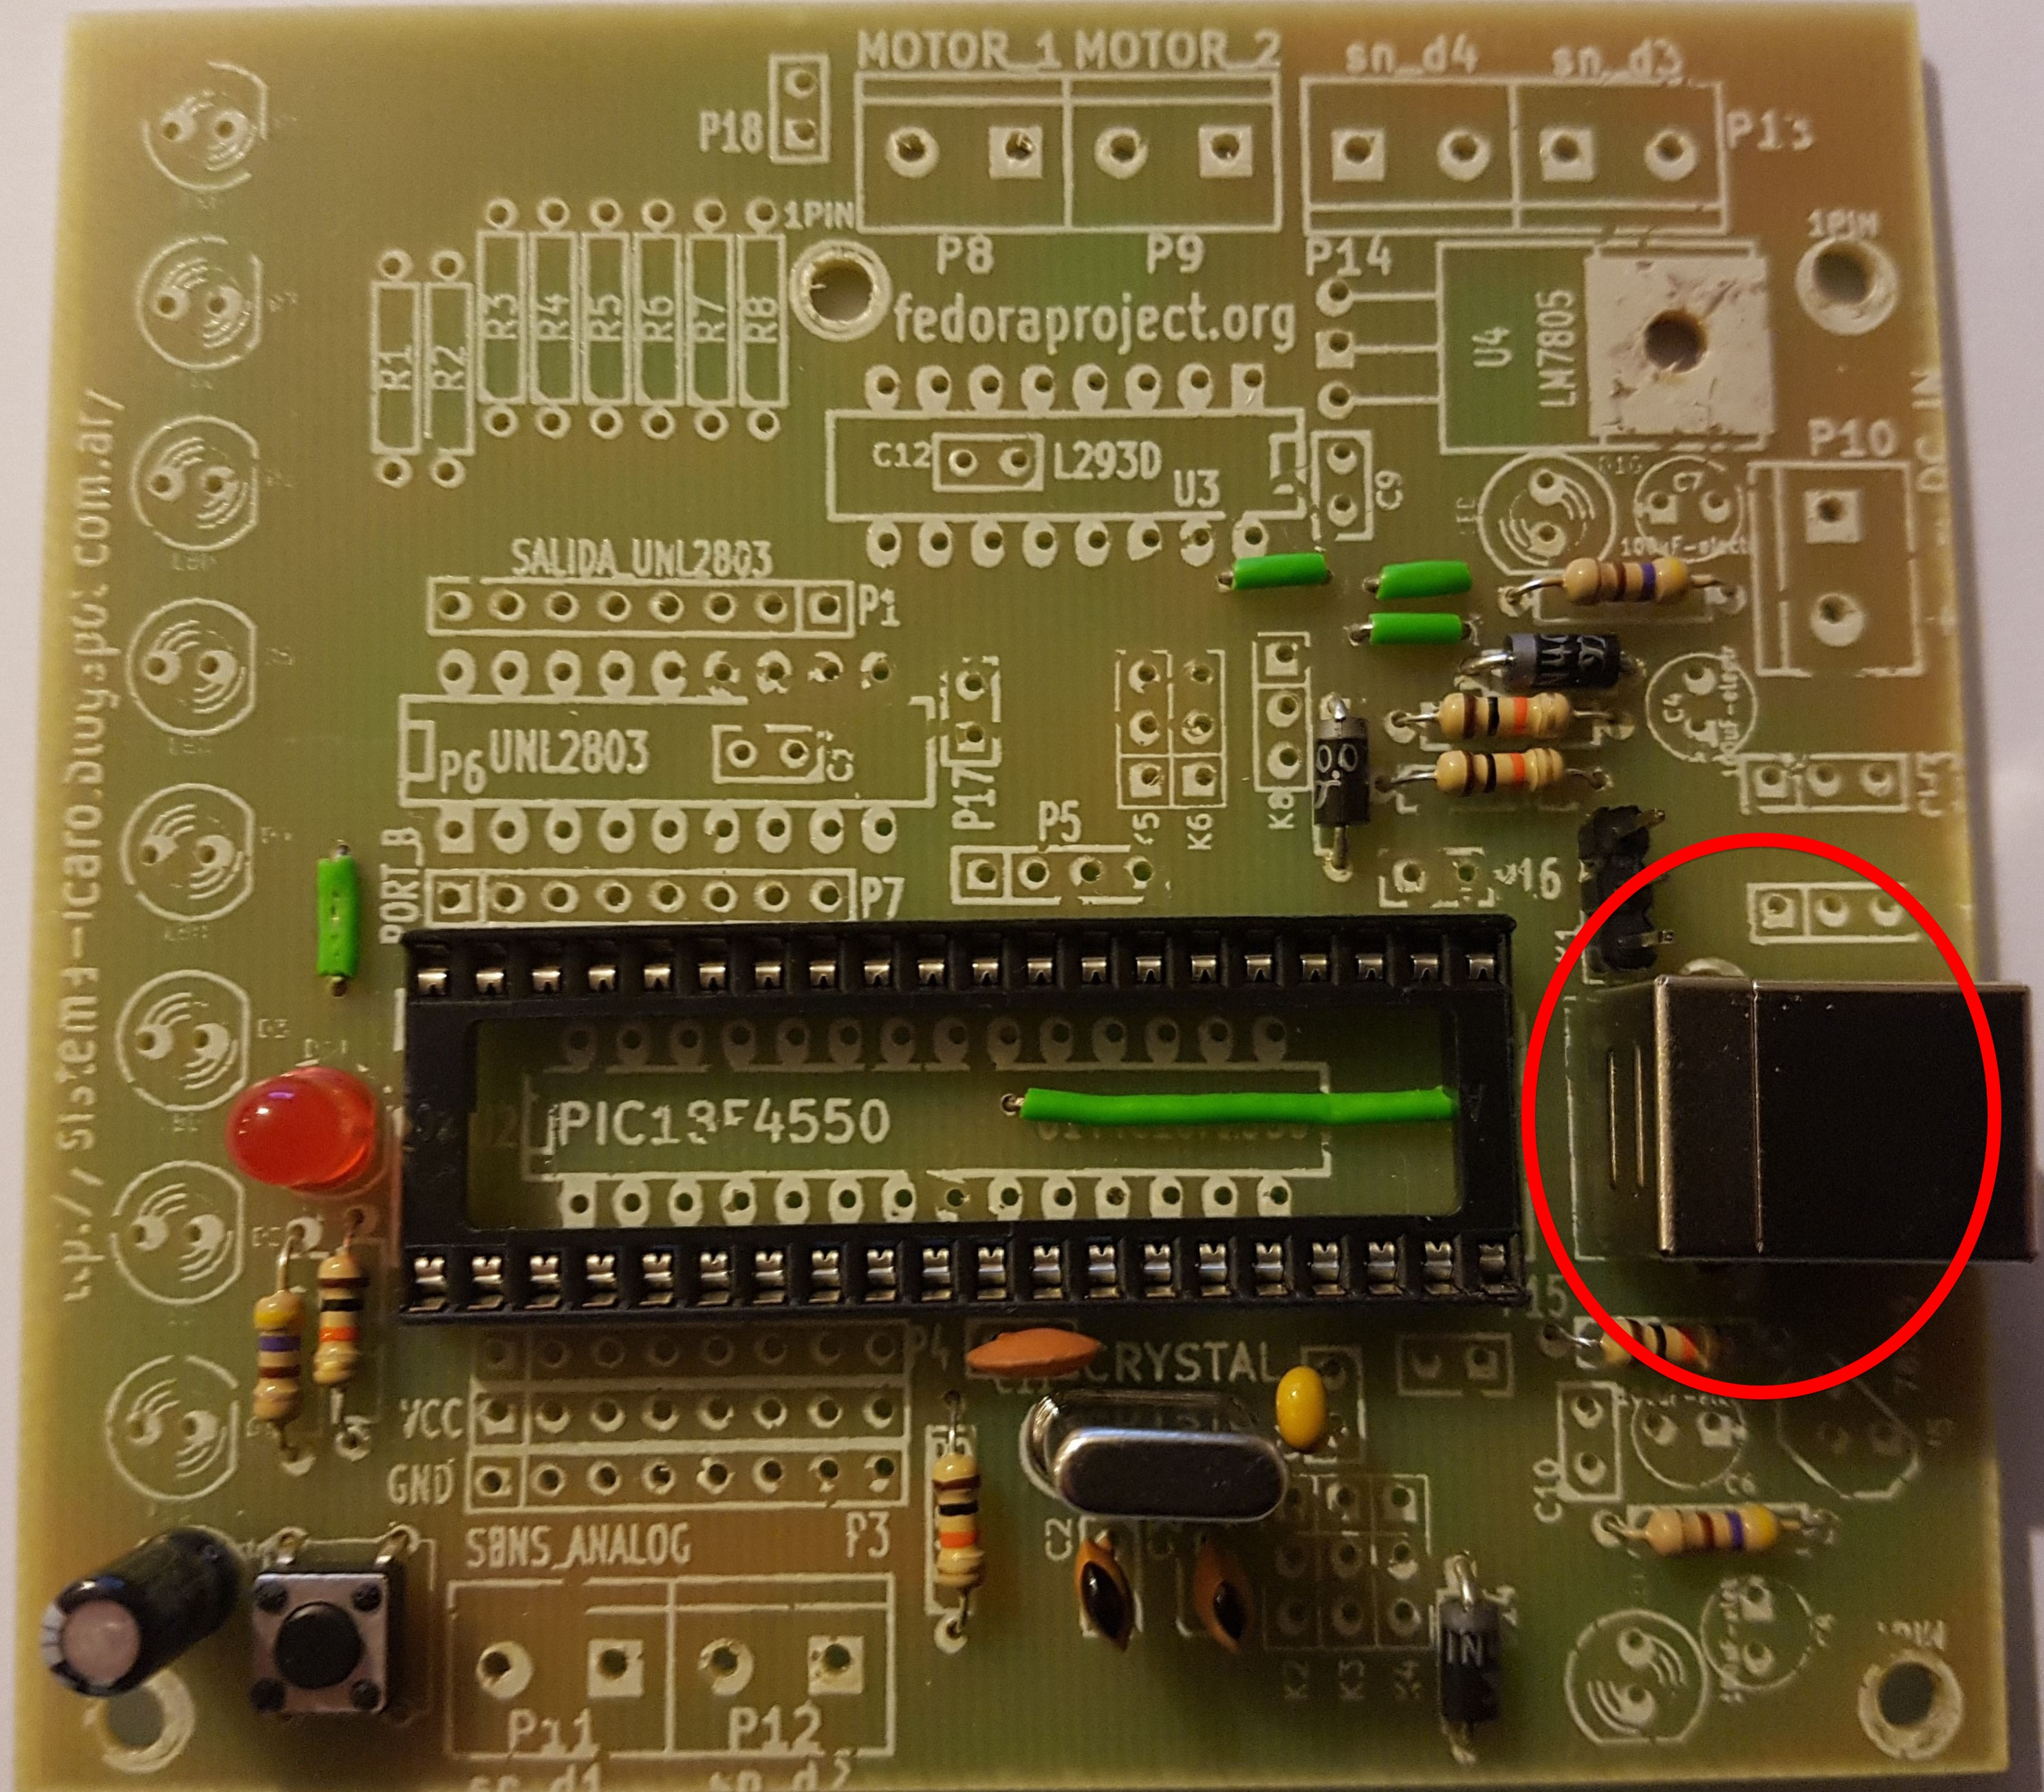
\includegraphics[width=0.8\linewidth]{Modulo_2/M2_10}
	\caption{Módulo 2 - Paso 10}
	\label{fig:M2_10}
\end{figure}

\newpage

\section{Paso 11:}

Instalar interruptor. SW1 y SW3. Opcionalmente se pueden usar pines machos

\begin{figure}[h]
	\centering
	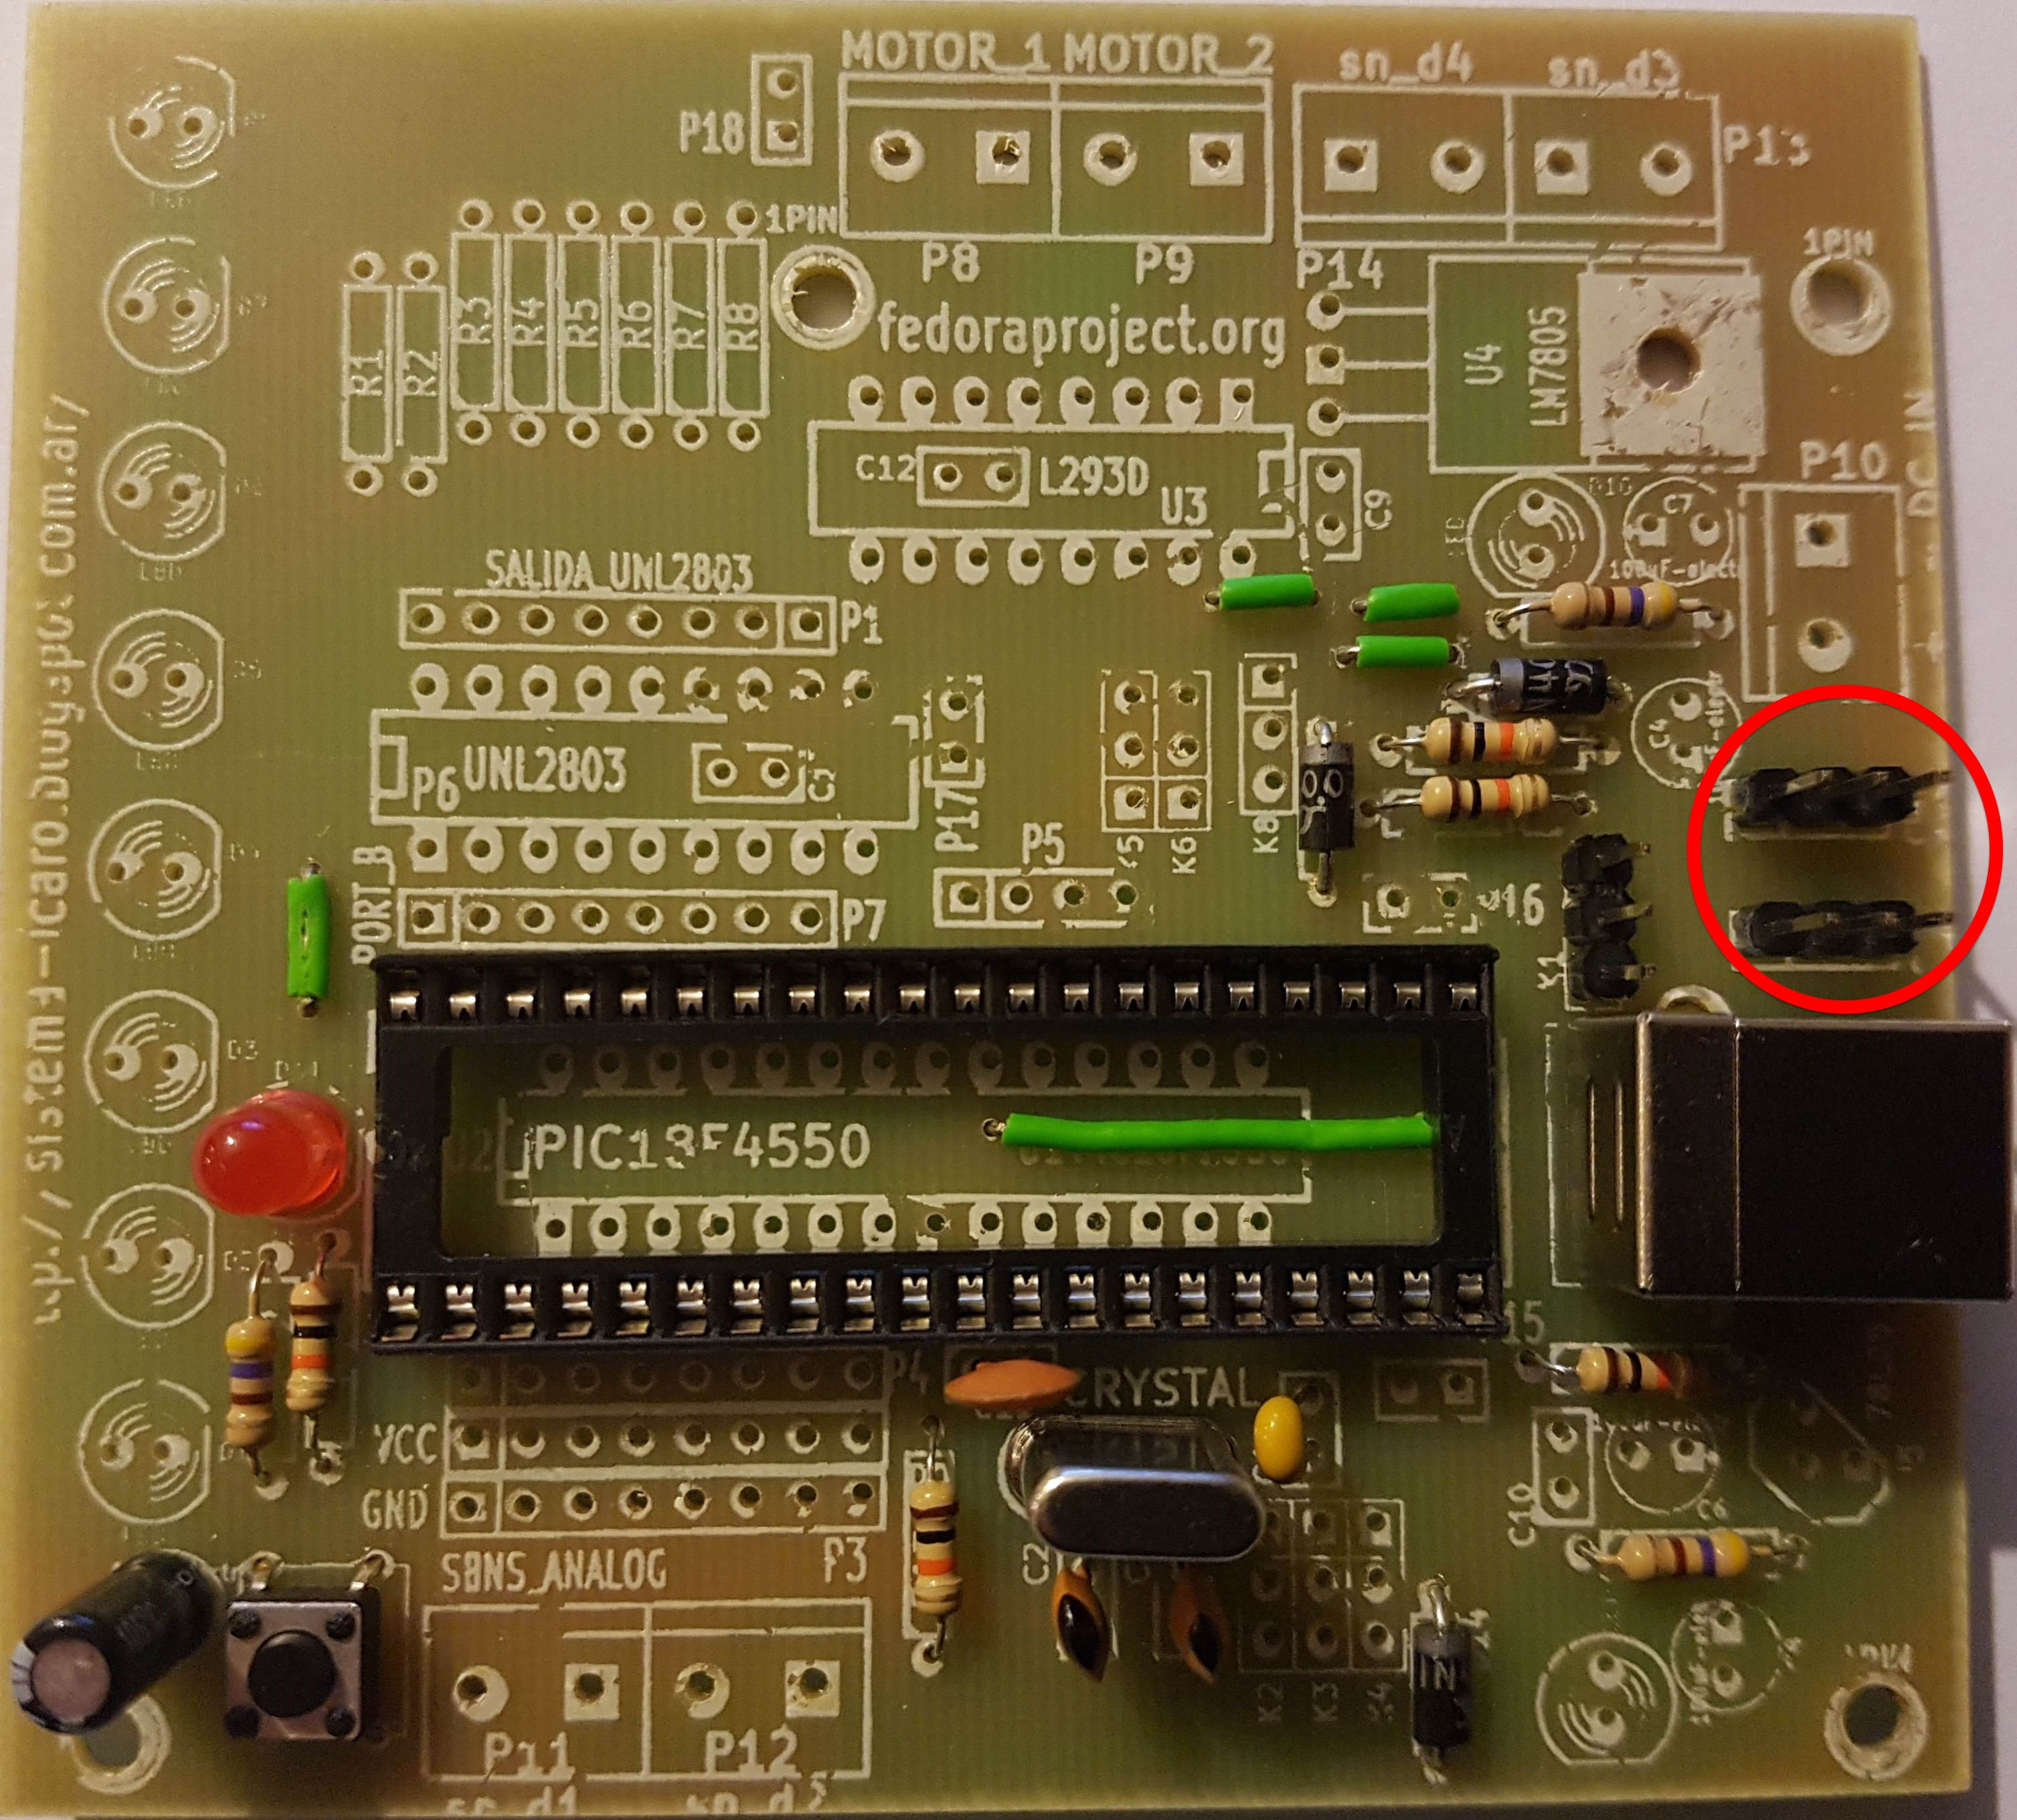
\includegraphics[width=0.8\linewidth]{Modulo_2/M2_11}
	\caption{Módulo 2 - Paso 11}
	\label{fig:M2_11}
\end{figure}

\newpage

\section{Paso 12:}

Instalar jumper en pines del lado del puerto USB en el selector K1

\begin{figure}[h]
	\centering
	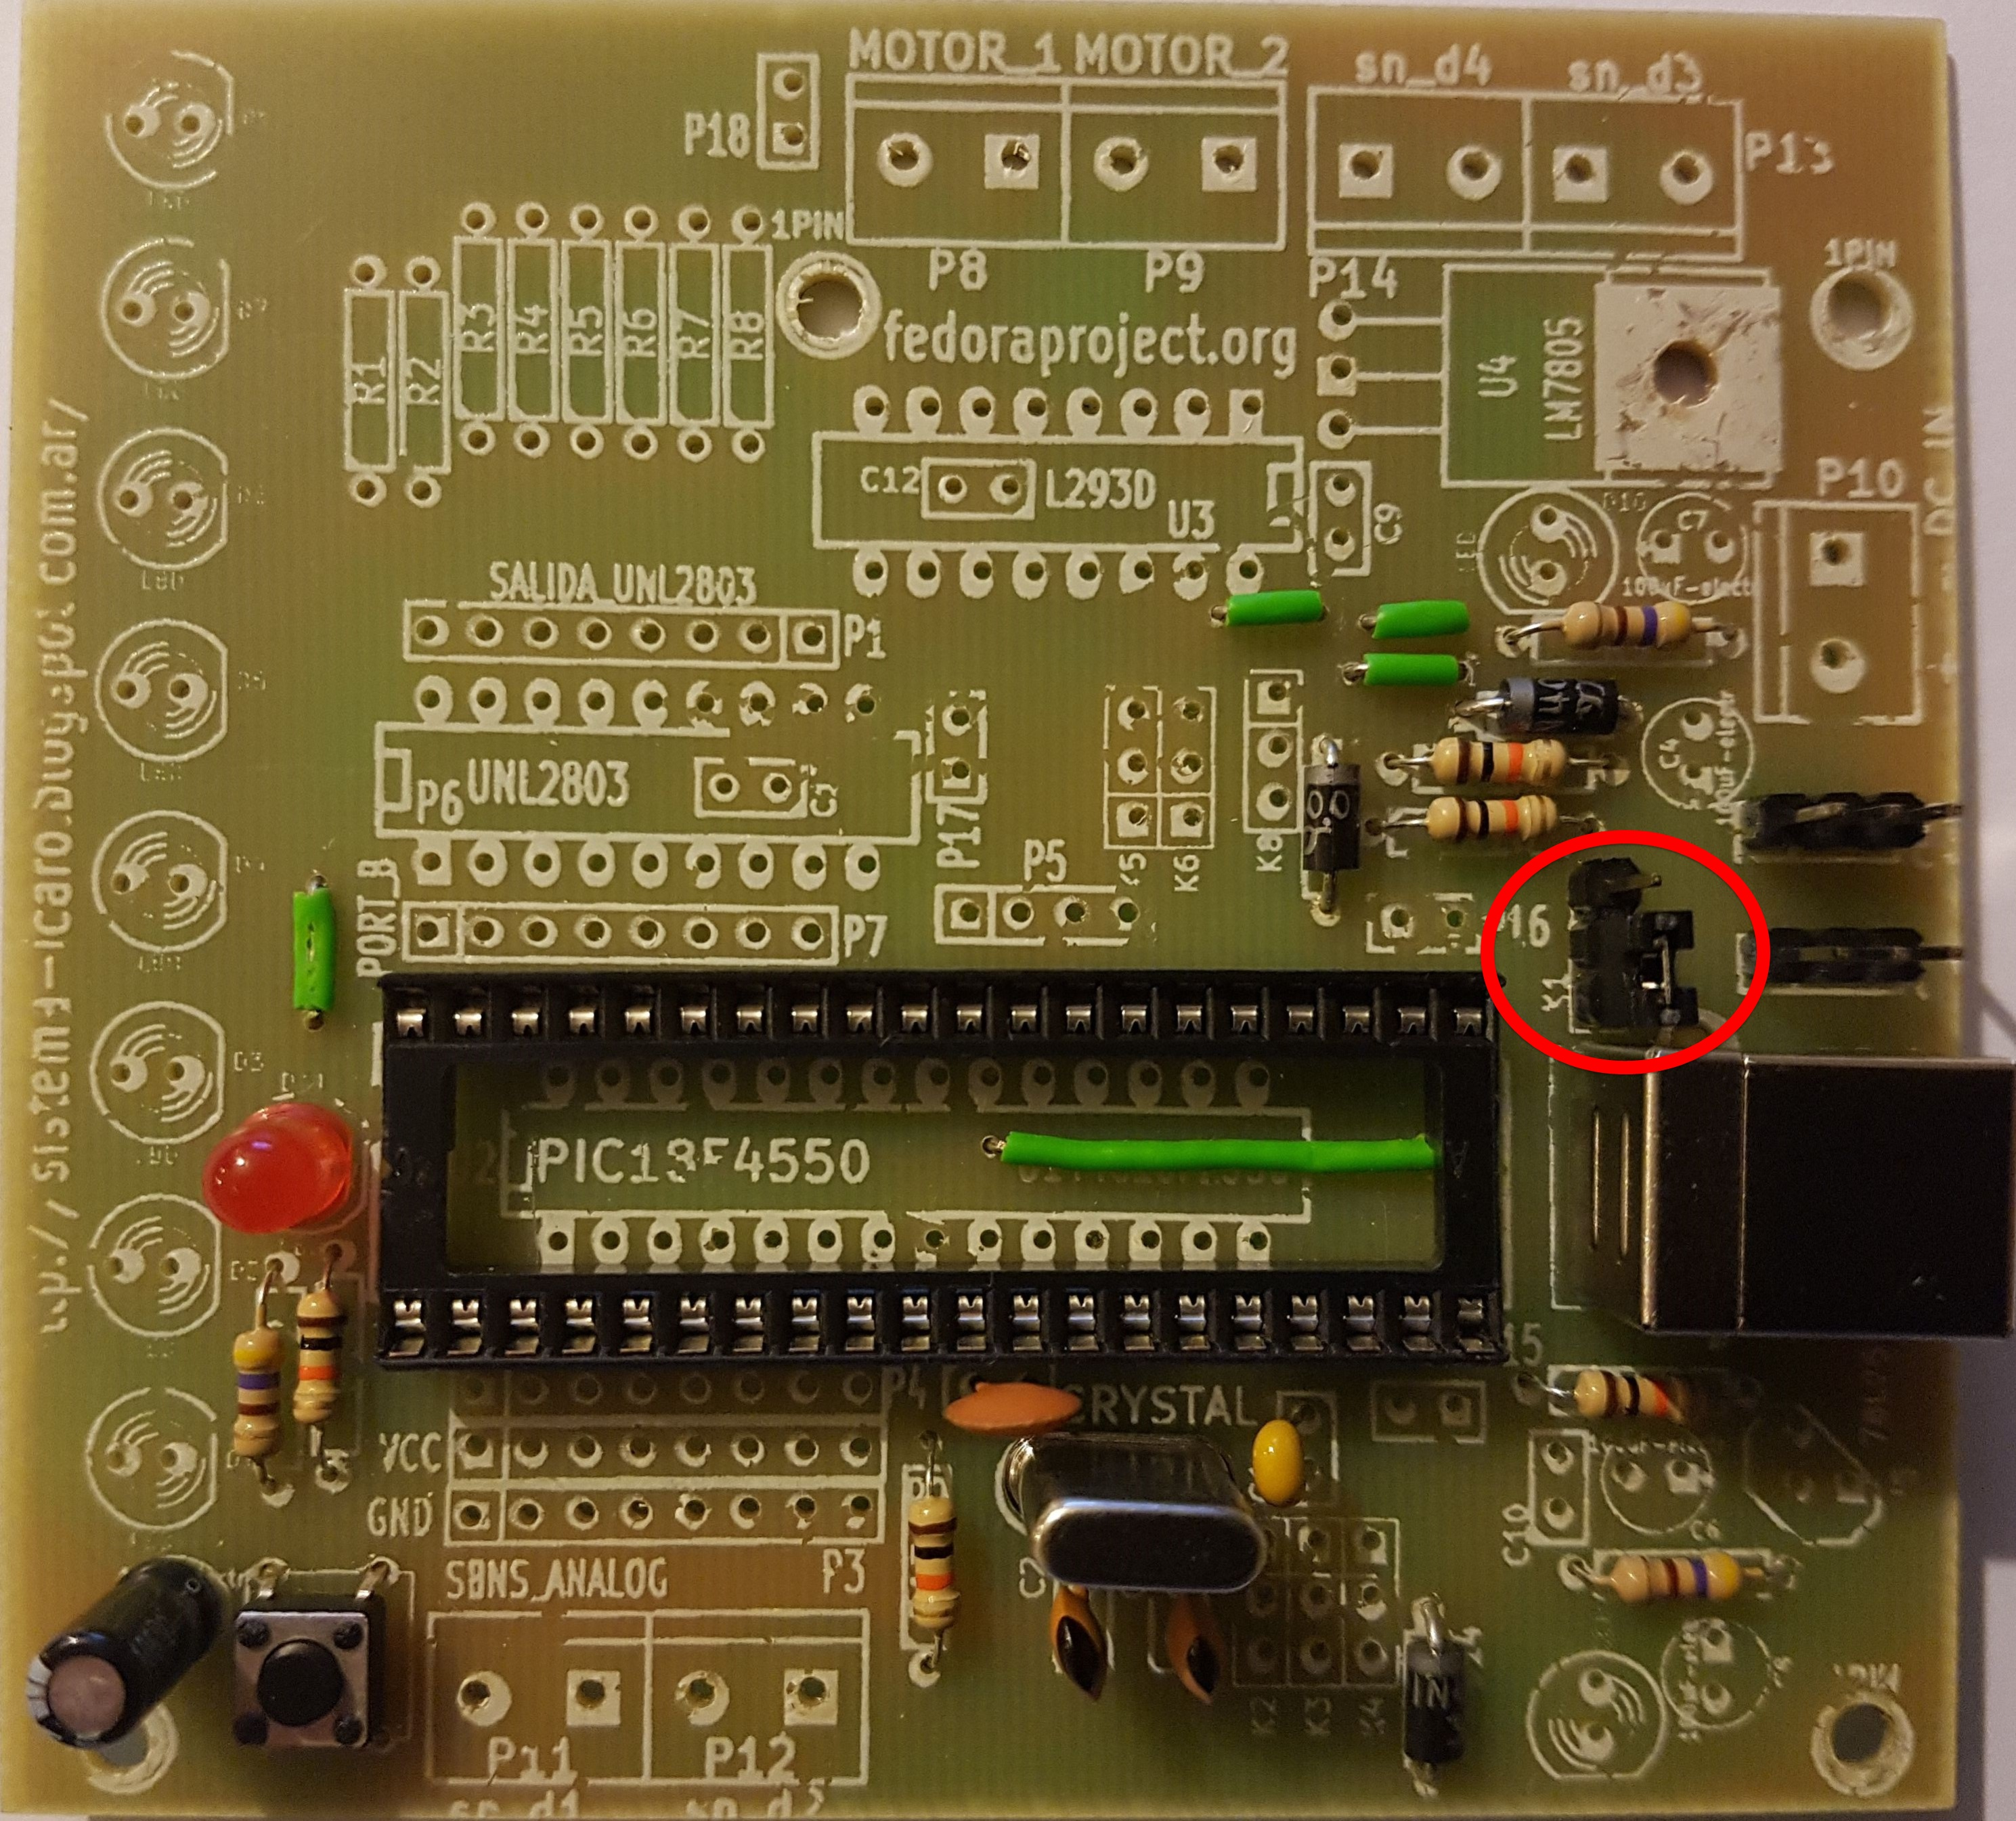
\includegraphics[width=0.8\linewidth]{Modulo_2/M2_12}
	\caption{Módulo 2 - Paso 12}
	\label{fig:M2_12}
\end{figure}

\newpage

\section{Paso 13:}

Instalar PIC 18F4550 en el Zócalo U2

\begin{figure}[h]
	\centering
	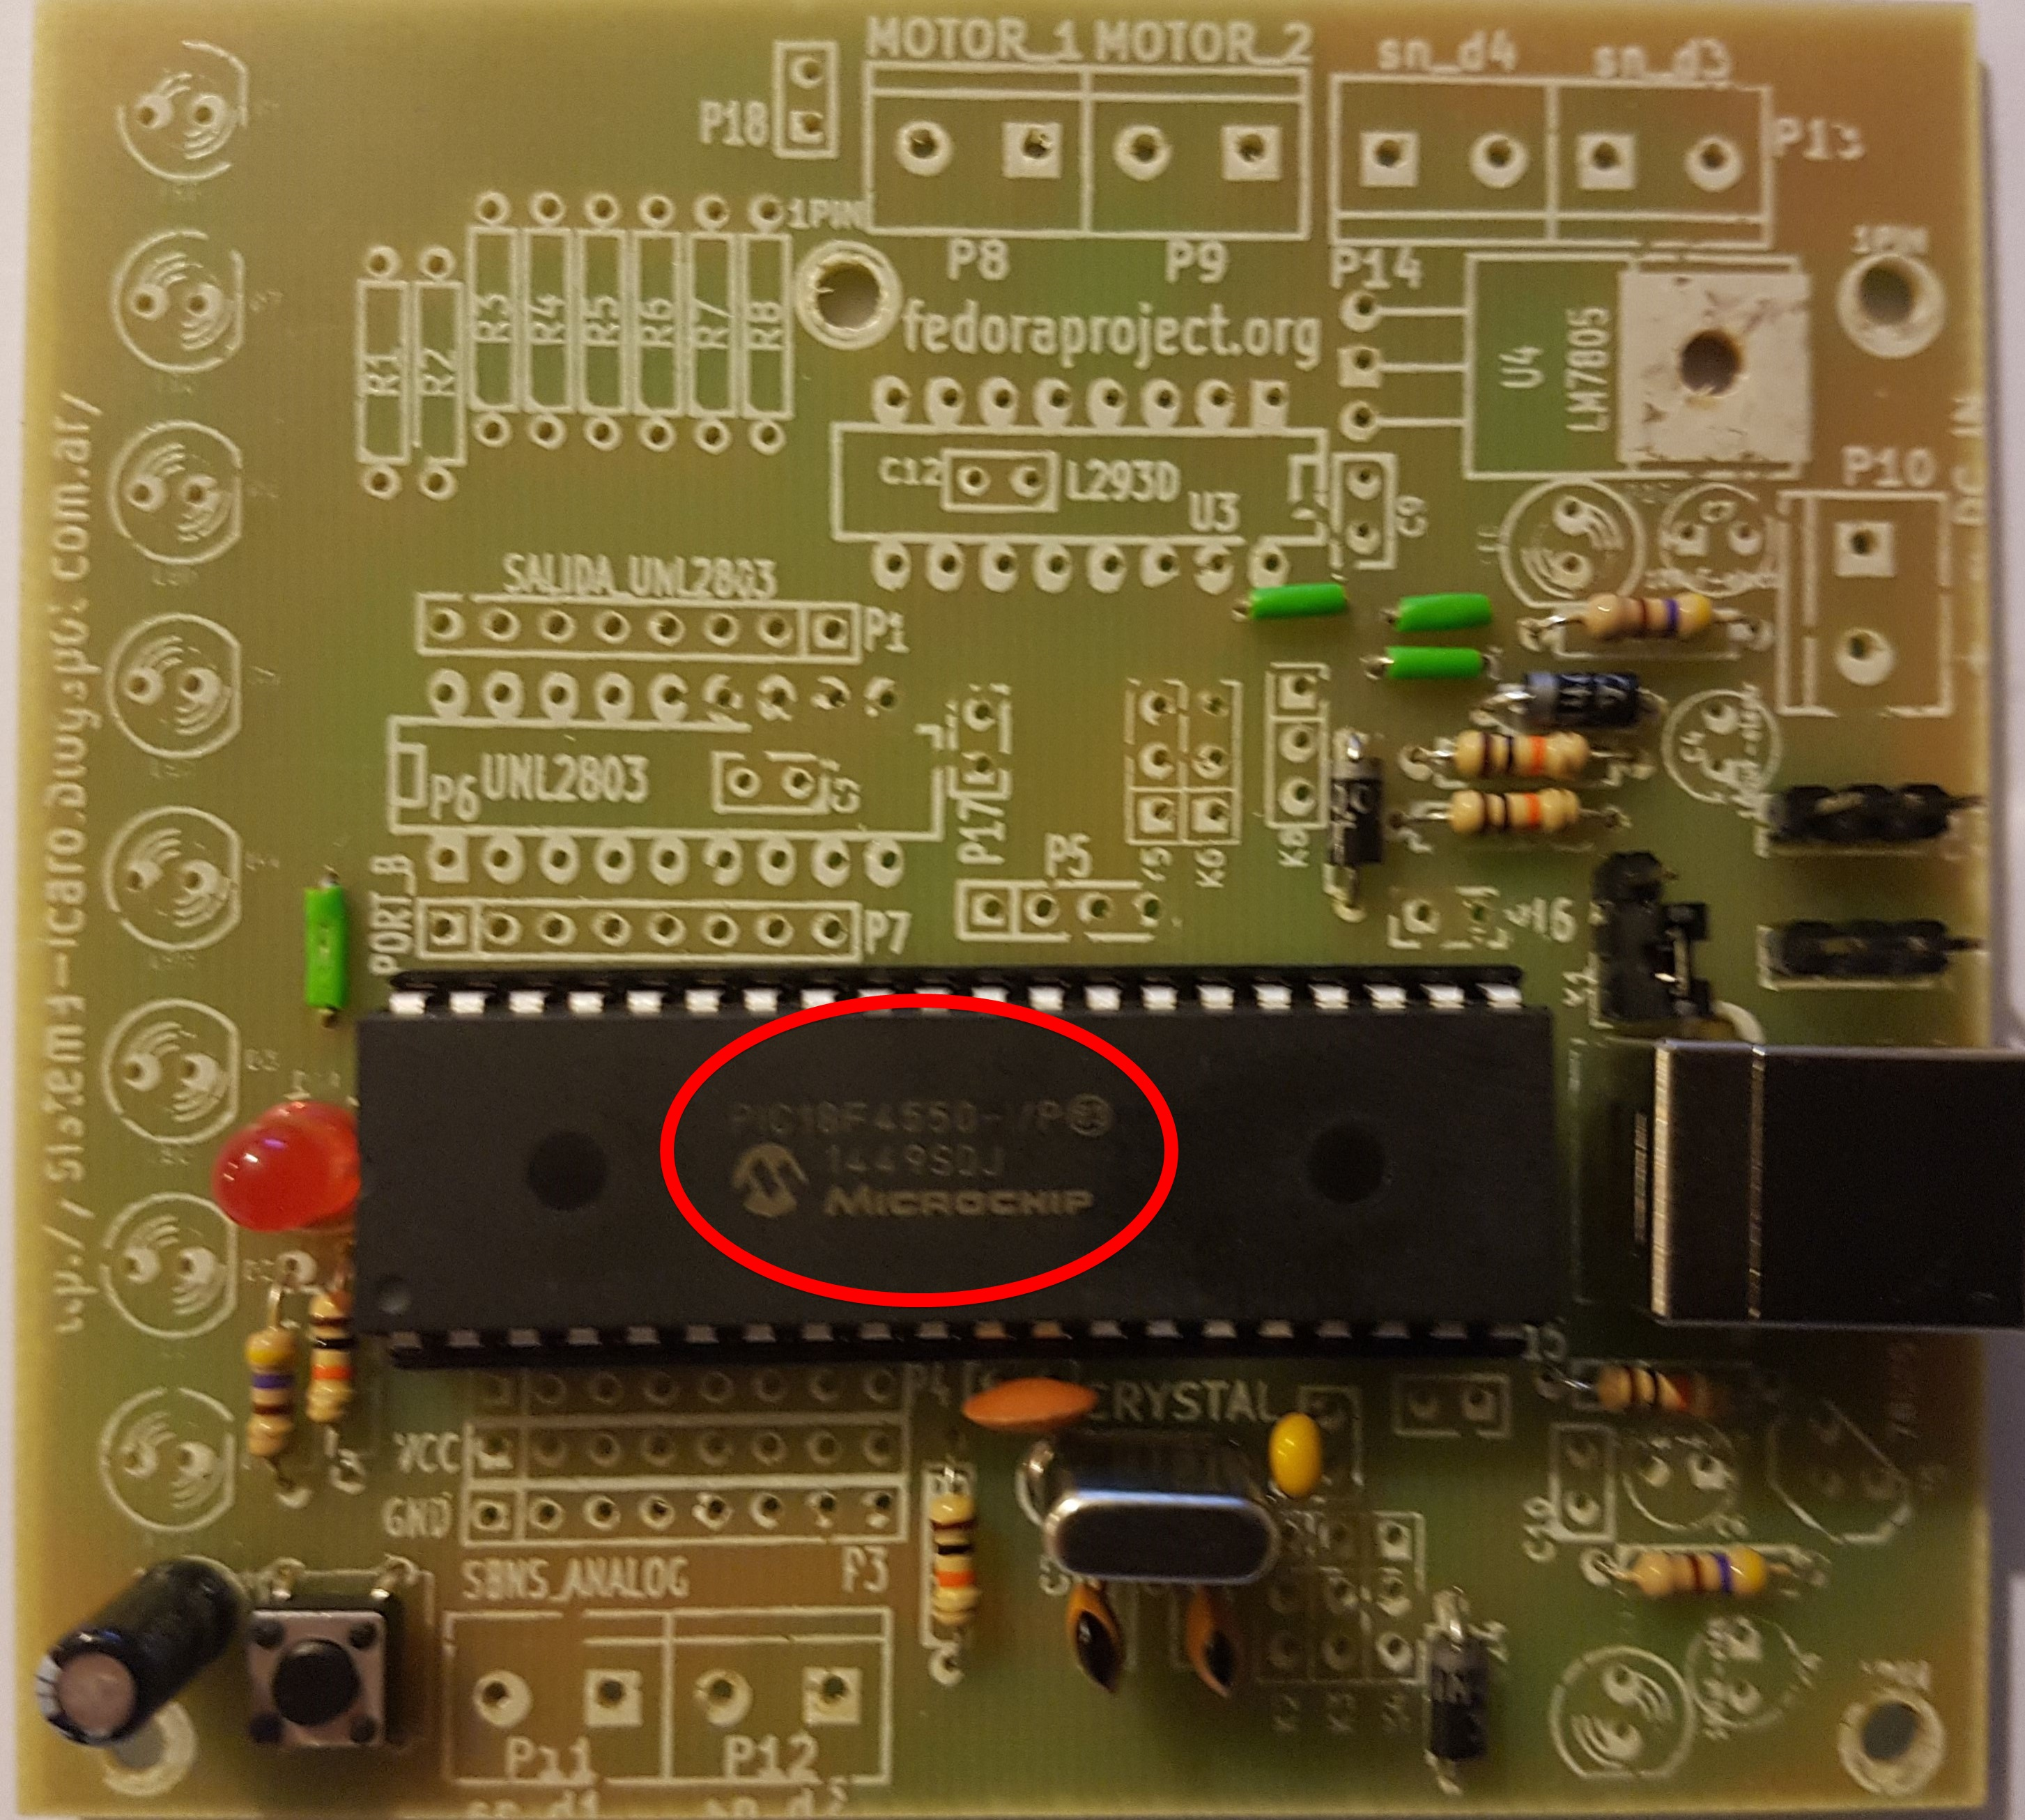
\includegraphics[width=0.8\linewidth]{Modulo_2/M2_13}
	\caption{Módulo 2 - Paso 13}
	\label{fig:M2_13}
\end{figure}

\newpage


NOTA: Las tiras de pines machos K5 y K6 podían instalarse en este momento para la comunicación con vía bluetooth HC-05. Para la comunicación solo se requieren los pines del lado del micro. Por comodidad se pueden instalar de una vez ambos puertos completos (los tres pines de cada puerto) y tener los pines para alimentación.

Comprobación
El puente al centro del micro debe dar +5VDC contra tierra.
El poner un micro con un script debe encender el led rojo D11

Nota: D11 no se enciende si el micro solo tiene el bootloader. Se puede cargar un programa en blanco de icaro bloques para probar que la placa levanta el micro. 

